




%\setlength{\parindent}{8pt}
\section{Introduction}
With the development of technology in modern society, more and more data can be recorded as a function in a time interval rather than as a scalar at a discrete time point. With the increasing capability and complexity of data emerged a new data type – functional data. Functional data abstract ordinary data into high dimensional data and apply it to a wider range of scenarios. This has boosted the advent and rise of functional data analysis (FDA) in recent years, which provides statistical methodologies to deal with functional data. Many techniques in the multivariate analysis have been extended to FDA and there are more and more works to perfect this field. In the book (Ramsay, Hooker, and Graves, 2009), he first introduced some preliminaries about functional data including mean function, bivariate function, and smoothing methods. After that, he covered a popular technique Functional Principal Component Analysis (FPCA), which is not straightforward but can be analogized with ordinary PCA. Finally, he put forward a functional linear model and deduced three ways to estimate the functional coefficients using the least square method. There are also methods from others to estimate such as the nonparametric method (Ferraty and View, 2006), and the partial least square approach (Preda, Saporta, and Lévéder, 2007). Apart from the model building in functional data, there are also techniques in the statistical test. Permutation t-test and permutation F-test based on Bootstrap (Ramsay, Hooker, and Graves, 2009) can test whether the difference between two groups or models is significant. Later, Cuesta-Albertos et al.(2019) proposed a goodness of fit on the functional linear model based on random projected empirical processes. The functional data analysis theories system is being improved year by year.

However, even though FDA has increased the complexity of the model from the perspective of data and may have improved performance in some scenarios, it is still mostly related to the linear model nowadays and could not explain some intricate relation between response and covariates. Thanks to the development of neural networks and the capability of networks to figure out intricate relations, we can combine neural networks and functional data to analyze complicated problems. Several works following the idea proposed different methods to realize this combination. Thind et al (2022) proposed a framework named FuncNN dealing with functional data with a neural network. It approximates infinite dimensional functional data using basis expansion with a prior basis and a number of bases. Then it takes the inner product of functional covariates and bases as input of the neural network and implements the following layers the same as the traditional one. However, a prior may greatly influence the performance of a model. AdaNN (Yao, Mueller \& Wang, 2021) proposes an adaptive basis layer instead of a fixed and given basis expansion. It learns the bases layer through an end-to-end pattern and the other parts of AdaNN are similar to FuncNN. 

Functional data analysis could be employed in many fields including air quality analysis, medical images, and even network service management. In their work (Martínez et al, 2014), they applied functional data analysis to detect outliers in air quality samples and compared the results from functional data analysis and classical methods. A shift-invariant model (Heinrichs, Heim \& Weber, 2023) provides a method for the classification of electroencephalography (EEG) data, a popular field of research in brain science using functional data analysis. It combines functional data analysis and convolutional neural networks to classify the medical images of brains from EEG data. In addition, functional data analysis could also be network management. Perdices et al (2021) characterized network services times series using functional clustering, augmented by autoencoder neural networks to improve the results. They exemplified the application in real cases and showed functional data analysis and neural networks are complementary. These applications in real scenarios represent the wide use and power of functional data analysis with neural networks. 


In this project, we first review methods from Ramsay et al (2009), compare their methods with the traditional multivariate method, and apply those methods to real data experiments. A by-product when comparing is a functional linear regression method called the functional score regression, which considers PCA on a multivariate perspective together with a functional linear model instead of FPCA with functional principal component regression. 

The rest of this project is organized as follows. Section 2 reviews those theories in FDA and Functional neural networks (Thind, Multani, and Cao, 2022). In Section 3, we collect data from the real scenario, implement the models in the data and compare the results of the models. Finally, we make a summary in Section 4, discussing the experiment and further work that need to be done.


\section{Materials and methods}

\subsection{Methodologies}
In this section, we introduce the theory of this experiment. Figure \ref{fig: flowchart} goes through the procedures of this experiment.\\
\numberwithin{figure}{section}
\begin{figure}[H] %H为当前位置,!htb为忽略美学标准,htbp为浮动图形
\centering %图片居中
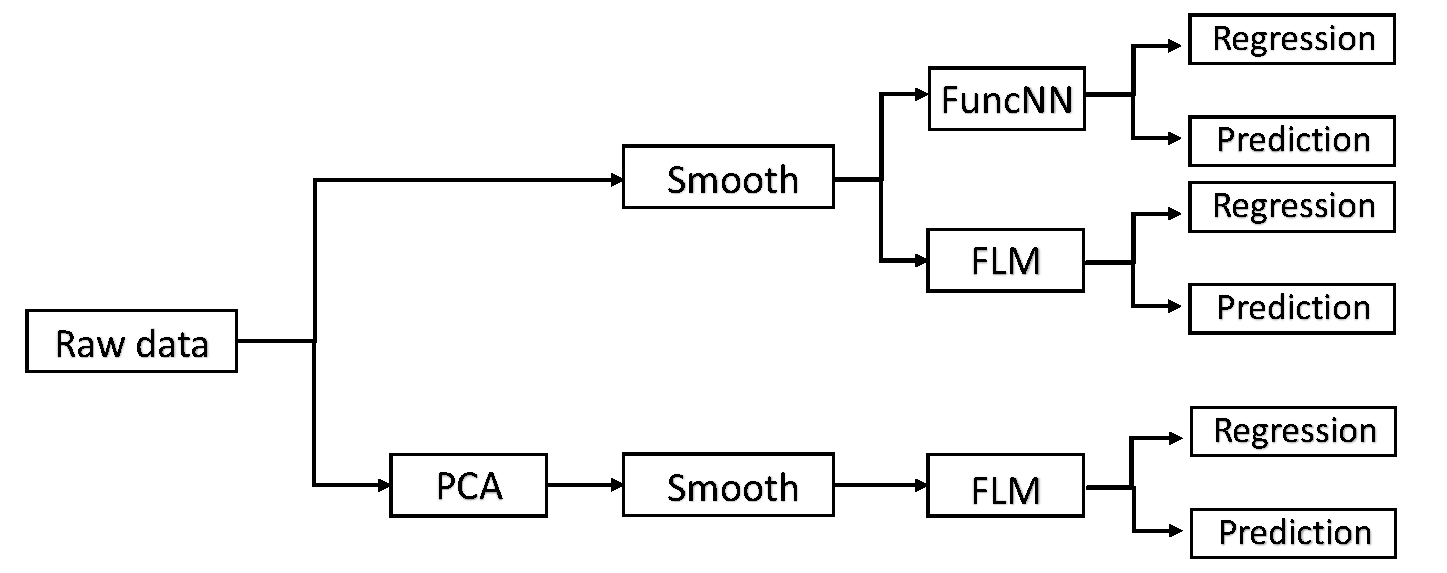
\includegraphics[width=1.0\textwidth]{3.1.pdf} %插入图片,[]中设置图片大小,{}中是图片文件名
\caption{Flow chart for the whole procedure} %最终文档中希望显示的图片标题
\label{fig: flowchart} %用于文内引用的标签
\end{figure}
\noindent
In our work, we first smooth the data by some basis function expansion and obtain functional data. Then we perform some preprocesses on those functional data pointwise. Apart from these basic preprocesses, a novel technique called Functional Principal Component Analysis (FPCA) is introduced and we also derive a new method named Functional Score Method. The upper panel shows the procedures of building a functional model, while the lower panel is the path that Functional Score Method goes through. Finally, we applied prepared data into a functional linear model and also a functional neural network. In addition, we compare the differences between functional models and their traditional models. 
 
\subsection{Data Smoothing}
Since the original data we got are discrete, to analyze with functional data, we need to transform those data into a functional form, which is called smoothing. The purpose of data smoothing is trying to find a function that the data exactly follow.  Smoothing can reduce noise and unnecessary details in the data, to better reveal the overall trend and pattern of the data. There have been several methods for data smoothing, including basis expansion and the nonparametric kernel method. Most of the works developed on functional data analysis using the method of basis expansion, as we do later. However, there are some precautions when we use basis expansion data smoothing. It assumes that we can find a finite number of basis functions to span the space of the true function we aim to approximate. While it may not be always true, since the function may be infinite-dimensional. We accept this assumption to adapt to further theories. For basis expansion data smoothing, functional data is usually expressed as a linear combination of basis functions, which have the following form,
\numberwithin{equation}{section}
\begin{equation}
x(t) = \sum\limits_{k=1}^K c_{k}\phi_{k}(t)= \bm c^{\prime} \bm\phi(t),
\label{func1}
\end{equation}
where $\bm c$ is the coefficient vector and $\bm \phi(t)$ is the vector of basis functions. Fourier Series and B-spline are two of the most commonly used basis types. We use the Fourier Series in the following since the Fourier Seris can extract cycle patterns in periodical data (Henderson, B. 2006). The Fourier Series functions are shown as follows: 
\begin{align*}
\phi_{1}(t) &= 1\\
\phi_{2}(t) &= \sin(\omega t)\\
\phi_{3}(t) &= \cos(\omega t)\\
\phi_{4}(t) &= \sin(2\omega t)\\
\phi_{5}(t) &= \cos(2\omega t)\\
&\quad  \vdots\\
wher&e \quad \omega = 2 \pi / T.
\end{align*}
The basis type and number of basis functions are always decided subjectively, we can estimate the coefficients by minimizing the following,\\
\begin{equation}
SSE\left(x\right)=\ \sum_{j}^{n}\left[y_j-x\left(t_j\right)\right]^2,
\label{func2}
\end{equation}
where $y_{j}$ is the observed value at time $t_{j}$ and $x(t_{j})$ is the smoothed data. After plugging function \ref{func1} into \ref{func2} we have,\\
$$SSE\left(\bm{c}\right)=\ \sum_{j}^{n}\left[y_j-\ \sum_{k}^{K}{c_k\phi_k\left(t_j\right)}\right]^2=\ \sum_{j}^{n}\left[y_j-\bm{\phi}\left(t_j\right)^\prime\bm{c}\right]^2.$$\\
$\bm \hat{c}$ can be solved by least square method:\\
$$\hat{\bm{c}}=\left(\bm{\Phi}^\prime\bm{\Phi}\right)^{-1}\bm{\Phi}^\prime\bm{y}.$$
The dimension of $\phi$ is $n \times k$ and the dimension of y is $n\times1$, where $n$ is the number of observations and $k$ is the number of basis functions.

Similar to the traditional linear model, we could also consider adding a penalty to the loss function shown in equation \ref{func2}, trying to avoid overfitting:
$$F\left(\bm{c}\right)=\sum_{j}\left[y_j-x\left(t_j\right)\right]^2+\ \lambda\int\left[Lx\left(t\right)\right]^2dt,$$
where $Lx(t)$ is a linear differential operator on $x(t)$ and $\lambda$ denotes the parameter of penalty.

We choose $L=\omega^2D+D^3$ since we are working on a group of periodical data with a known period, and this penalty can substantially penalize the high-order terms in the Fourier Series. We can see for any periodical data $a_{j}\sin(j\omega t)+b_{j}\cos(j\omega t)$ with known frequency $\omega$, its linear differential operator: 
$$L\left[a_j\sin{\left(j\omega t\right)}+b_j\cos{\left(j\omega t\right)}\right]=\omega^2j\left(1-j^2\right)\left[a_j\cos{\left(j\omega t\right)}-b_j\sin{\left(j\omega t\right)}\right].$$
We observe that when j = 1, there is no penalization. As j increase, the increase of penalty is proportional to $j^2 (1-j^2)^2$ which is very large. Thus, the penalty constricts the form into $a\sin(\omega t) + b\cos(\omega t)$.
\noindent
For the choice of $\lambda$, it can be determined by Generalized Cross Validation (GCV):\\
$$GCV\left(\lambda\right)=\left(\frac{n}{n-df\left(\lambda\right)}\right)\left(\frac{SSE}{n-df(\lambda)}\right).$$\\
For a fixed $\lambda$, we can get the following new loss function,\\
$$F\left(\bm{c}\right)=\sum_{j}\left[y_j-\bm{\bm\phi}^\prime\left(t_j\right)\bm{c}\right]^2+\lambda\bm{c}^\prime[L\bm{\phi}(t)L\bm\phi^{\prime}(t)dt]\bm c.$$
and then $\bm \hat{c}$ and $df(\lambda)$ can be calculated by the following:
$$\text{set}\quad \bm{R}=\int{L\bm{\phi}\left(t\right)L\bm{\phi}^\prime\left(t\right)dt},$$ 
then we can solve by the least square method: 
$$\hat{\bm{c}}=\left(\bm{\Phi}^\prime\bm{\Phi}+\lambda\bm{R}\right)^{-1}\bm{\Phi}^\prime\bm{y}.$$
If we design the hat matrix as:
$$\bm{H}=\bm{\Phi}\left(\bm{\Phi}^\prime\bm{\Phi}+\lambda\bm{R}\right)^{-1}\bm{\Phi}^\prime,$$
then the degree of freedom as a function of $\lambda$ can be calculated by: 
$$df\left(\lambda\right)=\mathrm{trace}\left[\bm{H}\left(\lambda\right)\right].$$

Finally, we introduce how we select the number of basis functions in the real precipitation data. While many works decide the number of basis functions subjectively, we determine the numbers according to some criterion. Too many basis functions may overfit the data, while too less could lose the information of the true function. Here, we choose a combination of AIC (Akaike Information Criterion) and BIC (Bayesian Information Criterion), their average, to select the number of basis functions. AIC and BIC are two indices that penalize the number of basis functions, which can help to avoid overfitting, so it can help us to choose the number of basis functions. However, in our data set, the number of basis functions of those five covariates can not be selected by AIC or BIC independently (e.g., the AIC or BIC for one of the covariates monotone increase or decrease), so we use the value of AIC + BIC as a criterion for the number of basis functions choosing problem.
$$AIC=2k+n\ln{\left(RSS/n\right)},$$
$$BIC=\ln{(n)}k+n\ln{\left(RSS/n\right)}.$$

\subsection{Preprocessing for Functional Data}
After smoothing the data, the following procedures are similar to the procedures of the traditional model. We also do data preprocessing on functional data. Similar to the univariate version, we have sample mean function and sample variance function pointwise. Sample mean function for functional data defined as:
$$\bar{x}\left(t\right)=N^{-1}\sum_{i}{x_i\left(t\right)},$$
where each $x_{i}(t)$ is a sample curve after smoothing, and $N$ is the number of curves. Sample variance function for functional data:
$$s\left(t\right)=\left(N-1\right)^{-1}\sum_{i}\left[x_i\left(t\right)-\bar{x}\left(t\right)\right]^2.$$
Similarly, each $x_{i}(t)$ is a sample curve after smoothing and $N$ is the number of curves.
After getting the sample mean function $\bar{x}(t)$ and sample variance function $s(t)$, we can scale the functional data point wisely,
$$x_i^\prime\left(t\right)=\ \frac{x_i\left(t\right)-\bar{x}\left(t\right)}{\sqrt{s\left(t\right)}}.$$

\subsection{Functional Principal Components Analysis}
The sample mean function and sample variance function are so straightforward that we can derive them from the conventional model point wisely. However, things seem quite different in the principal component analysis for functional data. For the conventional dataset, we can use a covariance matrix of covariates and decompose it to find eigenvectors. While the sample variance function defined before cannot be used to figure out eigenvectors. Instead, we need the covariate function of functional data and fortunately, it can be defined as a bivariate covariance function:\\
$$v\left(s,t\right)=\left(N-1\right)^{-1}\sum_{i}{\left[x_i\left(s\right)-\bar{x}\left(s\right)\right]\ \left[x_i\left(t\right)-\bar{x}\left(t\right)\right].\ }$$
Then the problem becomes how to decompose this covariance function since the dimension of this function is infinite. It is complicated to find eigenfunction in this way. Thanks to Ramsay et al. (2009), have developed a way to calculate the eigenfunctions from the other perspective. For conventional PCA model, suppose $\bm x_{i}\in R^p, i=1,\dots,n$ are $n$ observations with $p$ covariates after standardization, then we find eigenvector $\bm\xi \in R^p$ such that the variance of the inner product of $\bm x_{i}$ and $\bm \xi$ are maximized, namely solve eigenvector:\\
$$\bm{\xi}=\mathop{\arg\max}\limits_{\xi}\ \sum_{i}\left(\bm{x}_i\cdot\bm{\xi}\right)^2, \qquad \text{subject to  }  \bm \xi' \bm \xi = 1.$$
Then the result eigenvector $\bm \xi$  is the first principal component, and the other principal components are calculated similarly with additional constraints such that they are orthogonal to all the principal components found before. Borrowing this idea to functional principal component analysis, we expand observations $\bm x_{i}$ to functional observations $x_{i}(t)$, define probe function $\xi_{i}(t)$ or eigenfunction as the role of eigenvector $\bm \xi$, and realize inner product on $x_{i}(t)$ and $\xi_{i}(t)$ by integral $\int_{\mathcal{T}\ }{x_i\left(t\right)\xi_i\left(t\right)\mathrm{d}t}\,\ $ hence we aim to find a function such that:\\
$$\xi\left(t\right)=\mathop{\arg\max}\limits_{\xi}\ \sum_{i}[\int{x_i\left(t\right)\xi\left(t\right)\mathrm{d}t]^2},\qquad \text{subject to} \int\xi(t)^2\mathrm{d}t = 1. $$
In the same way, we can find other eigenfunctions with orthogonality constrain:\\
$$\int{\xi_i\left(t\right)\xi_j\left(t\right)dt}=0.$$

Here we only outline the basic idea to solve the eigenfunctions, but details to solve the problem especially how to find the function in an infinite dimensional space are not included. More details about the development and methods of FPCA are summarized by Wang, Chiou, and Muller (2015).

Although the procedures to figure out eigenfunctions or eigenvectors are similar, there are some differences between these two methods. PCA essentially takes a linear combination of covariates and extracts new covariates to do the dimension reduction. However, FPCA is not a dimension-reduction method for functional covariates. Instead, it can be used within only one functional covariate and output several eigenfunctions. These eigenfunctions, which may or may not be linear combinations of basis functions, can be treated as bases of sample space of that functional covariate. FPCA only explains the variance of samples within one functional covariate, it performs analysis on each functional covariate independently and was not extended to a linear combination of functional covariates. 

\subsection{Principal Component Score Function}
To apply the idea of PCA to functional data and solve the problem of multicollinearity, we propose a new method using PCA on functional data. We aim to find a function that we call score function: a linear combination of functional covariates such that:
$$sc\left(t\right)=\ \sum_{j=1}^{p}{\alpha_jx^{(j)}(t)}.$$
We mark different functional covariates with their superscripts, that is, $x^{(j)}$ represents $j-th$ functional covariates. Then the problem becomes how to figure out the coefficient $\bm \alpha$, and what the score function means. We use the eigenvector of data matrix $X$ as coefficient $\bm \alpha$, where $X$ is an $n\times p$ matrix whose $n$ rows represent $n$ observed times, and $p$ columns represent $p$ covariates. By using traditional PCA, we can solve out the eigenvector and hence $\bm \alpha$. Then for any given $t^{\prime}\in \mathcal{T}$, we can calculate $sc(t^{\prime})$ by $\bm \alpha$ and $x^{(j)}(t^{\prime})$. We see that $sc(t)$ is a function of $t$ and its value is derived from scores of principal components, thus we called it the score function. Notice that scores are obtained by eigenvector which maximizes the variance of the scores derived from $p$ covariates, then the first score function can be interpreted as the function varies most and explains the most variance of $p$ covariates. We use this score function as a new functional covariate to replace the original ones. In addition, we can find out more score functions through eigenvectors from PCA. 

\subsection{Functional Linear Model with Scalar Response}
The classical linear model gets the following form,
$$y_i=\ \sum_{j=0}^{p}{x_{ij}\beta_j}+\epsilon_i,\ i=1,\ \ldots,\ N$$
Now we assume that the response $y$ is a scalar and change at least one of the covariates into functional data, i.e., from $x_{i} =(x_{i1},\dots,x_{ip})$ to $x_i(t)$. We can choose different time points e.g., $t_{1},\dots ,t_{q}$ to get a model:
$$y_i=\alpha_0+\ \sum_{j=1}^{q}{x_i\left(t_j\right)\beta_j}+\epsilon_i.$$
If we select the time points finer enough, we can get a functional linear model as,
$$y_i=\alpha_0+\ \int{x_i\left(t\right)\beta\left(t\right)dt}+\epsilon_i.$$
More functional covariates can be added to the model as well as several scalar covariates. Generally, for an FLM model with $p$ scalar covariates and $q$ functional covariates, we have the following form,
$$y_i=\alpha_0+\bm{z}_{i}^\prime\bm{\alpha}+ \sum_{j=1}^{q}\int{x_{ij}\left(t\right)\beta_j\left(t\right)dt}+\epsilon_i,$$
where $\bm z_{i} = (z_{i1},\dots ,z_{ip})$ are the scalar covariates.

We aim to find coefficients $\bm \beta(t)$ and $\bm \alpha$. For the traditional scalar linear model, to estimate the coefficients, we can find the optimal solution to the loss function which is a function of scalar coefficients. However, for the functional linear model, it is not easy to estimate the optimal solution since some coefficients are functional and infinite dimensional. The loss function is expressed as $f(\bm\beta(t),\bm\alpha)$ which is not easy to find the derivatives and also the solutions. Thanks to the research in functional data analysis, there are ways to deal with the problem that function is infinite-dimensional. The basic idea is that assume functions can be approximated properly by a finite number of basis function expansions. From Ramsay et al.(2009), they express $\bm \beta(t)$ into linear combinations of basis functions, so that we can retrieve $\bm \beta(t)$ by solving
$$\beta\left(t\right)=\ \sum_{k}^{K}{c_k\phi_k\left(t\right)}=\bm{c}^\prime\bm{\phi}\left(t\right),$$
where $\bm\phi$ is a finite vector of basic functions. Then the loss function is expressed as a function of scalar inputs $\bm c$ and then the problem becomes finding out the coefficients vector $\bm c$ which optimizes the loss function.

To get the coefficients, similar to the classical linear model but apply the inner product to functional data, we aim to minimize the sum of square error (SSE) as the following term,\\
\begin{align*}
SSE\left(\bm \alpha,\beta\right)&=\sum_{i=1}^N\left[y_i-\bm{z}_{i}^\prime\bm{\alpha}-\sum_{j=1}^{q}\int x_{ij}\left(t\right)\beta_j\left(t\right)dt\right]^2\\
&=\ \sum_{i=1}^{N}\left[y_i-\bm{z}_{i}^\prime\bm{\alpha}-\sum_{j=1}^{q}c_{ij}\int x_{ij}\left(t\right)\phi_j\left(t\right)dt\right]^2,
\end{align*}
where $\phi_j$ is basis function expansion of $\beta_j,j=1,\ldots ,q$. To describe the solution more clearly, we express variables in matrix form. Define design matrix $Z$ as,\\
$$\mathbf{Z}=\left[\begin{matrix}\mathbf{z}_{1}^\prime&\int{x_{11}\left(t\right)\mathbf{\Phi}_{1}\left(t\right)dt}\ \ \ \ \ \ldots&\int{x_{1q}\left(t\right)\mathbf{\Phi}_{q}\left(t\right)dt}\\\vdots&\ddots\ &\vdots\\\mathbf{z}_{n}^\prime&\int{x_{n1}\left(t\right)\mathbf{\Phi}_{1}\left(t\right)dt\ }\ \ \ \ \ldots&\int{x_{nq}\left(t\right)\mathbf{\Phi}_{q}\left(t\right)dt}\\\end{matrix}\right]$$
where $\bm{\Phi}_{j},j=1,\dots,q$, is the vector of basis expansion, and here $ \bm {z}_{i}^\prime, i=1,\dots,n$ has its first element as 1 representing the intercept term.Define vector $\bm{y}=[y_1\cdots y_n]'$, and $\bm{b}=\left[\begin{matrix}\bm{\alpha}\\\bm{c}\\\end{matrix}\right]$, thus we have model:
$$\bm{y}=\bm{Zb}+\bm{\epsilon},$$
and the SSE:
$$(\bm{y}-\bm{Zb})'(\bm{y}-\bm{Zb}),$$
which can be solved by the least square method the same as the classical linear model. Then we can solve the coefficient matrix (including $\bm{\alpha}$ and $\bm c$) easily: 
$$\hat{\bm{b}}=\left(\bm{Z}'\bm{Z}\right)^{-{1}}\bm{Z}'\bm{y}.$$
Similar to smoothing, a functional linear model could also have penalties. Here we apply the Ridge penalty on functional covariates. The loss function with penalty is defined as:
$${\rm PENSSE}_\lambda\left(\bm \alpha,\bm \beta\right)=\sum\left[y_i-z_i'\alpha-\sum_{j}\int{x_{ij}\left(t\right)\beta_j\left(t\right)dt}\right]^2+\lambda\left(\int{\left[L \bm \beta'\left(t\right) L\bm \beta (t) \right]^2dt}\right),$$
where $L$ is the linear differential operator, and for the ridge method, it specializes as an identity operator. It is still the same for scalar covariates with its $L_2$ norm. $\lambda$ can be specified as different values for each covariate including functional and scalar ones. To solve the coefficients, we have the penalty matrix: \\
$$\left[\begin{matrix}\lambda_0 I &\ldots&\ldots&\ldots\\0&\lambda_1R_1&\ldots&0\\\vdots&\vdots&\ddots&\vdots\\0&0&\ldots&\lambda_qR_q\\\end{matrix}\right],$$
 where $R_j$ is the penalty matrix corresponding to the $j-th$ covariate $(j=1,\ldots,q):$ 
$$\bm{R}_j=\int{\bm{\phi}_j\left(t\right){\bm{\phi}_j}^\prime\left(t\right)dt}.$$
Then we can solve out the coefficient by normal function and the solution given by:$$\hat{\bm{b}}={\left(\bm{Z}^\prime\bm{Z}+\bm{R}(\bm{\lambda}\right))}^{-{1}}\bm{Z}^\prime\bm{y}.$$

\subsection{Functional Score Regression} 
As said before, FPCA only works with each functional covariate, to combine those functional covariates linearly, we propose the principal component score function method in Section 2.5. Functional score regression (FSR) is similar to a functional linear model and the only difference is that FSR replaces the original functional covariates of FLM with several principal component score functions obtained by PCA on multivariate data. To distinguish with FPCA regression, we called this method functional score regression (FSR).

\subsection{Functional Linear Model with Functional Response}
The functional linear model can also deal with the functional response using a concurrent model that is estimating functional response by the covariates at the same time points. The model can be described as:
$$\bm{y}(t)=\bm{Z}\left(t\right)\bm{\beta}(t)+\bm{\epsilon}(t),$$
where $\bm y(t)$ is a functional vector with length $N$ containing $N$ functional response and $\bm Z(t)$ is a functional covariate matrix with dimension $N\times p$. The loss function is similar but only replaces the square term with the inner product on the vector. Then solve the regression by normal equations:
$$\left[\int{\bm{\Theta}^\prime\left(t\right)\bm{Z}^\prime\left(t\right)\bm{Z}\left(t\right)\bm{\Theta}\left(t\right)dt}+\bm{R}\left(\bm{\lambda}\right)\right]^2\hat{\bm{b}}=\left[\int{\bm{\Theta}^\prime\left(t\right)\bm{Z}^\prime\left(t\right)\bm{y}\left(t\right)dt}\right].$$
where $\bm\Theta(t)$ is the basis function matrix of functional weight $\bm \beta(t)$, and  $\hat{\bm b}$ is the corresponding coefficient scalar vector.

\subsection{Functional Neural Networks with Scalar Response}
Functional Neural Networks got lots of similarities to Artificial Neural Networks (ANN), so we will first illustrate the implementation methods of ANN, and then generalize it to the Functional Neural Network.

An ANN is made up of neurons and their corresponding weights. It consists of some hidden layers, which contain several neurons. Each neuron in the layers is the output value of an activation function with a linear combination of previous neurons as input. More precisely, we can formulate as \\
$$\bm{v}^{(i)}=g\left(\bm{W}^{\left(i\right)}\bm{v}^{\left(i-1\right)}+\bm{b}^{\left(i\right)}\right),$$
where $\bm v^{(i)}$ is the neuron vector of $i-th$ hidden layer (original input is denoted as $\bm v^{(0)}$), $\bm W^{(i)}$ is the weight matrix from layer $i-1$ to layer $i$, and $\bm{b}^{(i)}$ is a constant vector referred as bias. g($\cdot$) is an activation function, which provides nonlinear transformation and can better describe the nonlinear model.

The training process of the network most frequently uses the backpropagation algorithm (Rumelhart, Hinton, and Williams, 1985). The algorithm first initializes the weights of the network and then spreads forward to calculate values in the output layer. After that is the backward process which updates weights by the gradient of the loss function calculated from the output value in the forward process. Repeat the forward and backward process until the loss decrement is small or some other criteria are met.

If we do not consider functional data, and treat all the observations of functional data as input directly into ANN. This kind of network is easy to understand but with some disadvantages. The first one is that the dimension may be large, however, this may not be severe for a network. The second one is about the interconnection within a functional covariate. If the real function is continuous, any two points infinitely close to each other would have value within a small neighborhood. While in practice, we only obtain finite data points and directly inputting them into the network may not conform to the characteristic. The third one is related to the interpretation of weight function. In this network, we do not care about the feature of the weight function whether it is continuous or not. Since the update process only considers the weight separately instead of treating them as a whole function. Hence, it may not ensure the feature of function such as continuity and smoothness.
\numberwithin{figure}{section}
\begin{figure}[H] %H为当前位置,!htb为忽略美学标准,htbp为浮动图形
\centering %图片居中
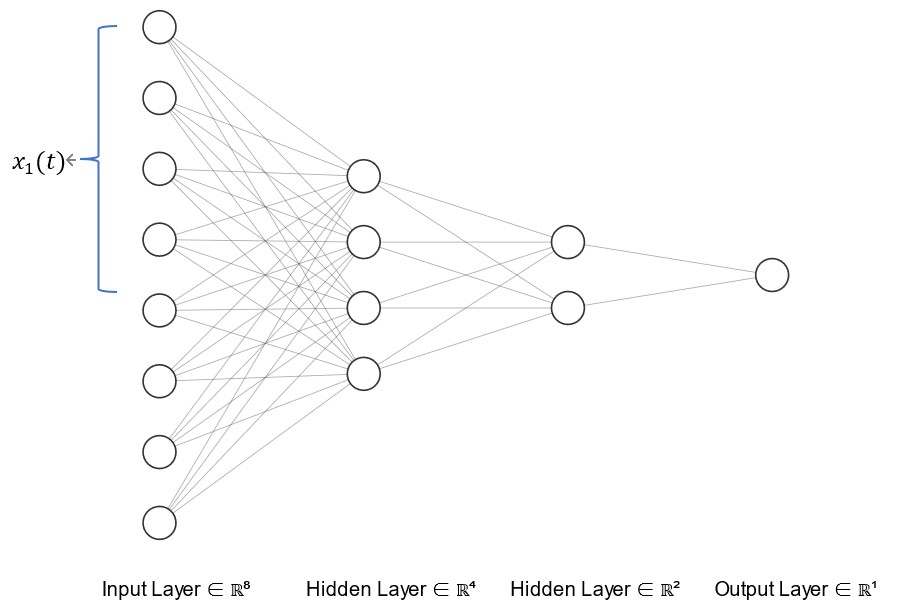
\includegraphics[width=1.0\textwidth]{fnn1.jpg} %插入图片,[]中设置图片大小,{}中是图片文件名
\caption{Traditional neural network structure} %最终文档中希望显示的图片标题
\label{fig: fnn1} %用于文内引用的标签
\end{figure}
%\ref{fig: flowchart}

Then we introduce functional data into the network. The first idea is that we can treat all data from one covariate together and share the same weight. Every neuron in the input layer records a single value at a time point of a functional covariate. The neurons in the red box represent one functional covariate, and each neuron in the next layer has only one shared weight which is a scalar. This kind of network does treat the input data as a whole but still does not explain the weight as functional. It only uses one value to weigh a functional input, which may not be accurate enough.
\numberwithin{figure}{section}
\begin{figure}[H] %H为当前位置,!htb为忽略美学标准,htbp为浮动图形
\centering %图片居中
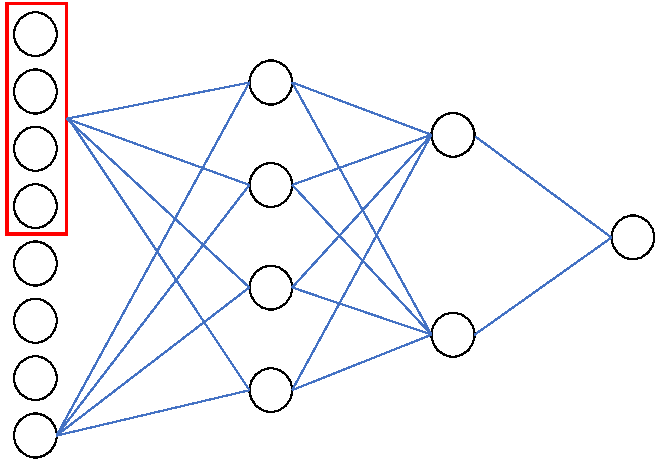
\includegraphics[width=0.8\textwidth]{fnn2.pdf} %插入图片,[]中设置图片大小,{}中是图片文件名
\caption{Functional neural network with shared weight} %最终文档中希望显示的图片标题
\label{fig: fnn2} %用于文内引用的标签
\end{figure}
%\ref{fig: flowchart}
The second network is to consider all the neurons as functional data rather than a scalar (scalar neuron can be treated as a constant function). Then the following picture shows the structure. The first layer is the input layer containing functional and scalar inputs. The weights are shown in blue segments which mean scalar weights. Since the linear combination of functions is still a function, then the activation function shown in green should be a map from function to function which is complicated. Then the output can be certainly functional. The weights are also scalar, while the neurons are all functional. It seems more general but is harder to implement since the activation function becomes more complicated.
\numberwithin{figure}{section}
\begin{figure}[H] %H为当前位置,!htb为忽略美学标准,htbp为浮动图形
\centering %图片居中
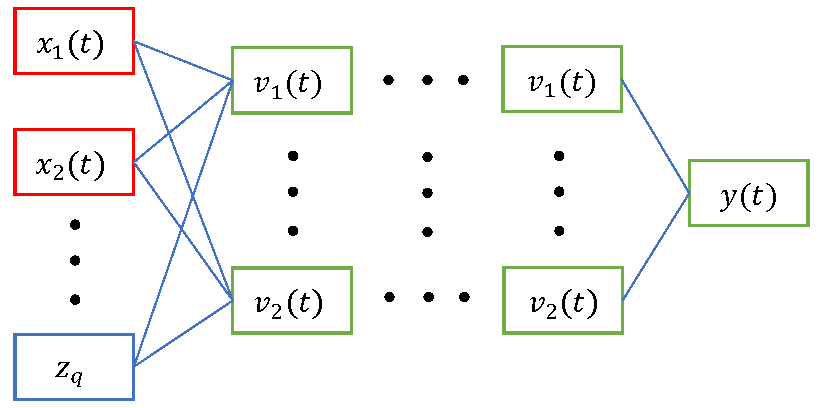
\includegraphics[width=0.9\textwidth]{fnn3.pdf} %插入图片,[]中设置图片大小,{}中是图片文件名
\caption{Functional neural network with functional neurons} %最终文档中希望显示的图片标题
\label{fig: fnn3} %用于文内引用的标签
\end{figure}
%\ref{fig: flowchart}

The last idea comes from Thind et al. (2022), who call their method FuncNN and do some transformation of functional data into the first layer. The graph below shows rough ideas of his work. Neurons in the first column colored in red represent functional covariates and all the others that are scalars are shown in blue. In this network, the weights colored in orange are functional and can be expressed as basis expansion. Multiplication of functional covariates and their corresponding weight functions is done by the inner product of two functions. Now that the inner product produces scalar outputs and so are the later part, which means that we can apply the rules of ANN to the later part of this network.
\numberwithin{figure}{section}
\begin{figure}[H] %H为当前位置,!htb为忽略美学标准,htbp为浮动图形
\centering %图片居中
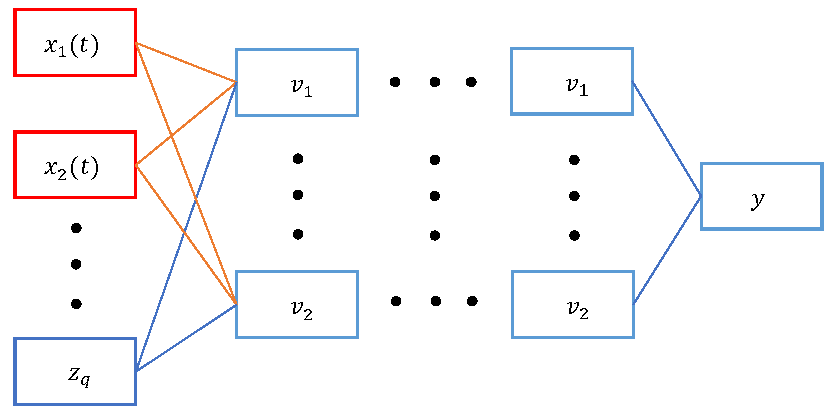
\includegraphics[width=0.9\textwidth]{fnn4.pdf} %插入图片,[]中设置图片大小,{}中是图片文件名
\caption{Functional neural network with functional weight} %最终文档中希望显示的图片标题
\label{fig: fnn4} %用于文内引用的标签
\end{figure}
\noindent
We can formulate the neurons in the first hidden layer by:
$$
v_i^{(1)} = g\Big(\sum_{k=1}^K \int_\mathcal{T}\beta_{ij}(t)x_k(t)\mathrm{d}t + \sum_{j=1}^Jw_{ij}^{(1)}z_j + b_i^{(1)}\Big),
$$
where $\beta_{ik}(t)$ is the weight function, $x_k(t)$ and $z_j$ represent functional and scalar covariates respectively, and $g(\cdot)$ is an activation function. 

The only difference between ANN and FuncNN is that FuncNN makes some transformation of functional data in the first layer and can use several scalars to represent weight functions. Details about the transformation from each functional covariate to different neurons in the first hidden layer and relevant weight functions are shown in the following Figure \ref{fig:fnn5}.
\numberwithin{figure}{section}
\begin{figure}[H] %H为当前位置,!htb为忽略美学标准,htbp为浮动图形
\centering %图片居中
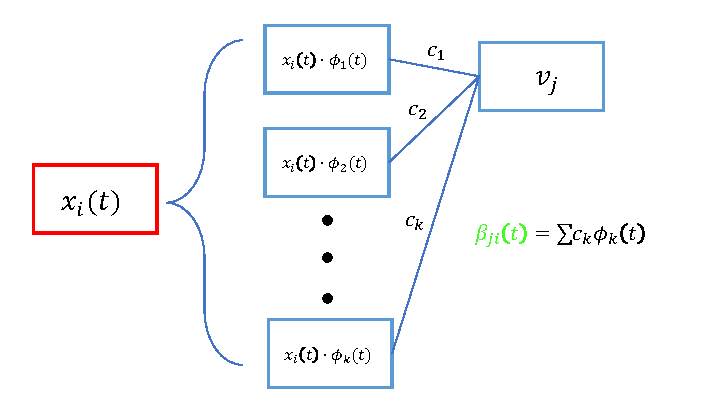
\includegraphics[width=0.7\textwidth]{fnn5.pdf} %插入图片,[]中设置图片大小,{}中是图片文件名
\caption{Details implemented in FuncNN} %最终文档中希望显示的图片标题
\label{fig:fnn5} %用于文内引用的标签
\end{figure}
%\ref{fig: flowchart}
From this figure, we can have a more specific view of how the weight function $\beta_{ji}(t)$ is obtained and the connection between ANN and FuncNN. Given hyperparameter $k$ and basic functions $\bm \phi^\prime$, the weight function can be spanned by
$$\beta_{ji}\left(t\right)=\sum c_k\phi_k\left(t\right).$$
Hence, the inner product of two functions can be expressed by:
$${\color{red}{x_i\left(t\right)}}\cdot{\color{green}{\beta_{ji}\left(t\right)}}=\sum c_k{\color{cyan}{x_i\left(t\right)\cdot\phi_k}},$$
where $x_i(t)\cdot\phi_k(t)$ are the input neurons in the first layer of ANN and coefficients $c_k$ correspond to weight $w_{ik}$ in ANN. Then we can show the formula of neurons in the first hidden layer in terms of basis functions $\phi_k$:
$$
v_i^{(1)} = g\Big(\sum_{j=1}^J \sum_{k=1}^{K}\int_\mathcal{T}\phi_{ijk}(t)x_j(t)\mathrm{d}t + \sum_{j=1}^Jw_{ij}^{(1)}z_j + b_i^{(1)}\Big).
$$
After applying the rules of ANN, we can figure out coefficients and hence weight functions through basis expansion.

This kind of network has treated functional input as a whole and can ensure some properties of weight functions by assuming basic functions. It is also easy to implement since most of the network is the same as the traditional ANN model. What’s more, it seems surprising that FuncNN uses fewer parameters than ANN that directly takes all observed data as input. Suppose $x_i(t)$ has $n$ observed time points, and we set weight function of FuncNN is spanned by $k$ basic functions. Then for ANN, the number of input neurons will be $n$, while for FuncNN, the number will be only $k$ according to the above, where $n$ should be larger than $k$. Thus, FuncNN appears to be more reasonable and efficient to deal with functional data.

As said before, most of the rules in ANN can also be adapted into FuncNN. We then consider some methods to complete the FuncNN model. For the training process, the backpropagation algorithm is still the most frequently used technique, and it is also applied to FuncNN. Furthermore, overfitting is also a common problem in neural network models since the number of parameters of the network seems not easy to determine. Thanks to the works on neural networks, two methods dealing with overfitting problems, drop out method (Srivastava et al., 2014) and early stop (Yao, Rosasco, and Caponnetto, 2007) method, have been utilized in FuncNN. More details about these two methods will be explained later in Section 3. 

\subsection{FuncNN with Functional Response}
FuncNN can also deal with the functional response and its method is quite straightforward if we know how to deal with functional covariates. It still expresses weight functions to functional response as basis functions expansion, takes the inner product of response and basis functions as output neurons, trains the network, and finally output coefficients indicating the weight functions.

\section{Results and Comparison}
In this section, we apply the theories above to a real scene using weather-related data from Macao SAR. We first briefly describe the data, and the methods of preprocessing data and then specify the model's hyperparameters we are going to build. Finally, we compare the results from different models including Functional Linear Model, Functional Score Model, and Functional Neural Network. 

\subsection{Data}
We utilize 24 years of weather-related daily data from Macao SAR, China, ranging from January 1, 1999, to December 31, 2022, download from \href{https://www.smg.gov.mo}{Macau Meteorological and Geophysical Bureau}. The dataset comprises daily average temperature, daily average relative humidity, daily average wind speed, daily average sea level pressure, daily total sunshine duration, and daily average precipitation.
Since there are few days of rain in a year, having precipitation data is not suitable to be regarded as functional data, we only consider daily average precipitation as a scalar response. The primary objective of this project is to use daily average temperature, daily average relative humidity, daily average wind speed, daily average sea level pressure, and daily total sunshine duration to conduct regression on yearly average precipitation. What’s more, we also use those 5 functional covariates stated above, adding yearly average precipitation at the current year as a scalar covariate, and predict the yearly average precipitation for the next year.

\subsection{Data Smoothing}
For each of the five covariates, we determine the number of basic functions by finding out the minimum value of AIC + BIC, and the corresponding number of basis is the one we want. We first calculate the value of AIC + BIC in a wide but sparse range, i.e., the basis number starts from 15 and ends at 365, while the gap equals 10. We will find an interval that may include the minimum value of AIC + BIC from that sparse interval, and further calculate the value of AIC + BIC on a dense interval, which got 50 points (50 different numbers of basis) with a gap equal to 2 (since Fourier basis function usually contains sine and cosine, so each time we need to add 2 more basis functions). The following graphs show the value of AIC + BIC corresponding to the number of basis functions.

\begin{figure}[H]
\centering  %图片全局居中
\subfigure[]{
\label{Fig.temp1}
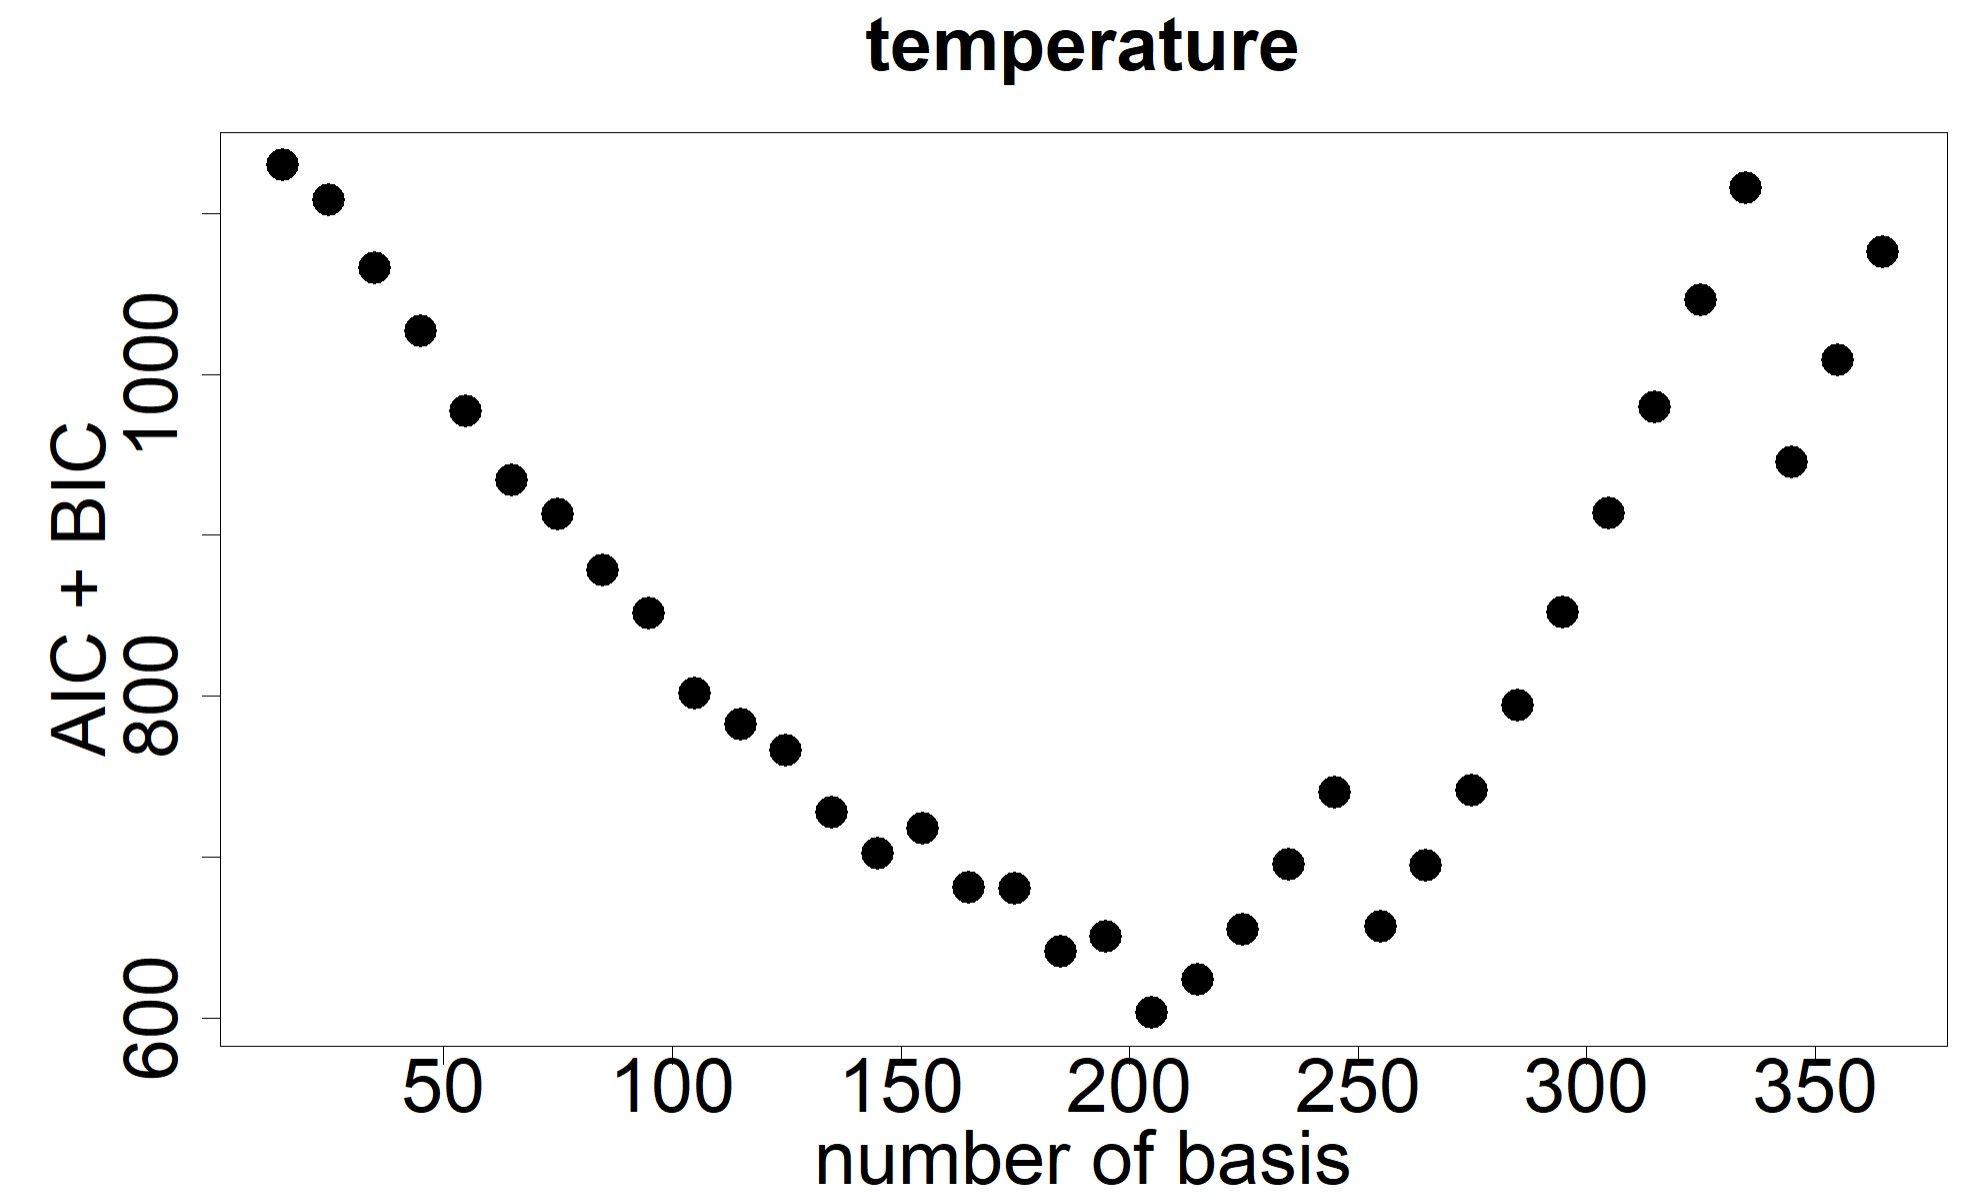
\includegraphics[width=0.47\textwidth]{temp1}}
\subfigure[]{
\label{Fig.temp2}
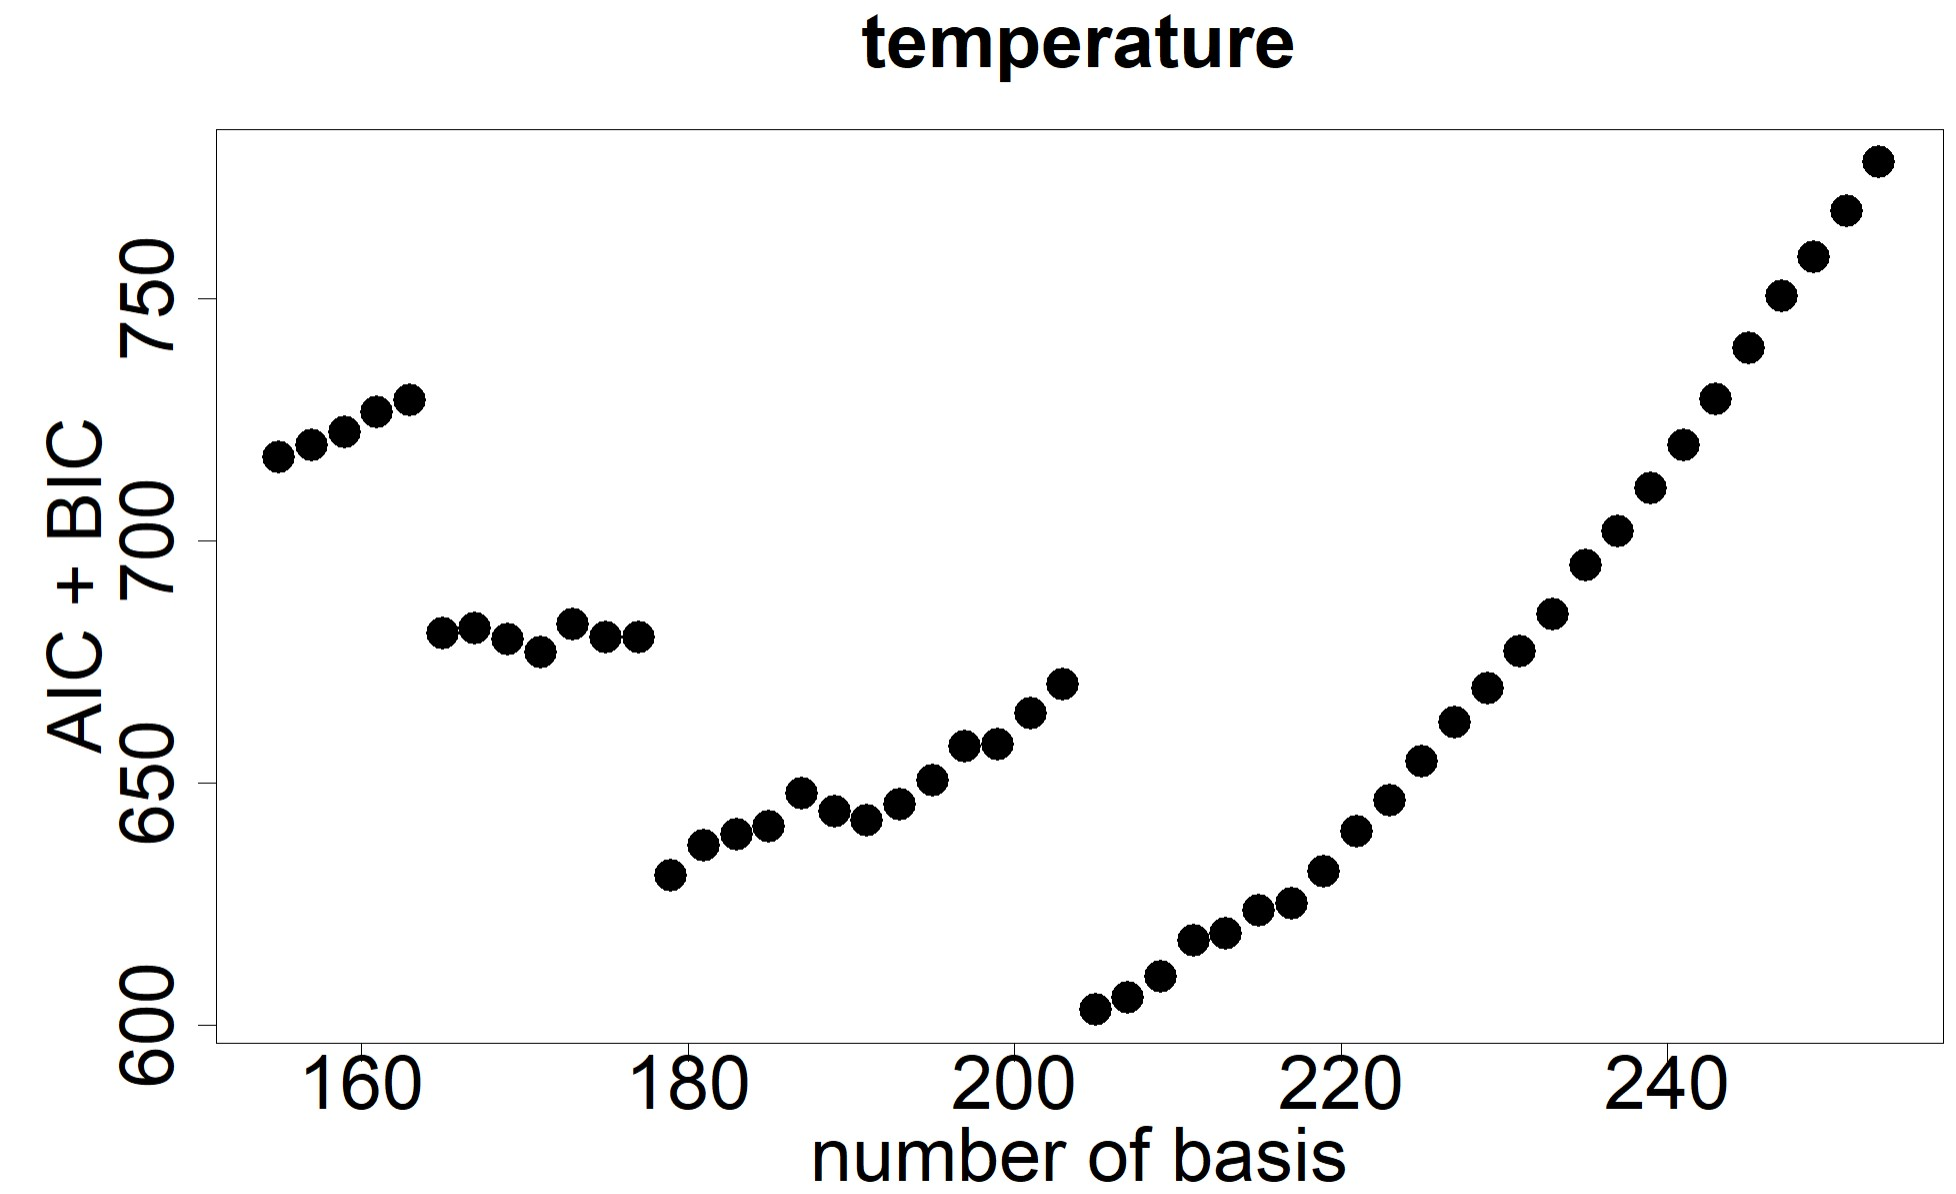
\includegraphics[width=0.47\textwidth]{temp2}}
\caption{The value of AIC + BIC corresponding to each $\log_{10}(\lambda)$ for Temperature}
%\label{Fig.main}
\end{figure}

\begin{figure}[H]
\centering  %图片全局居中
\subfigure[]{
\label{Fig.pressure1}
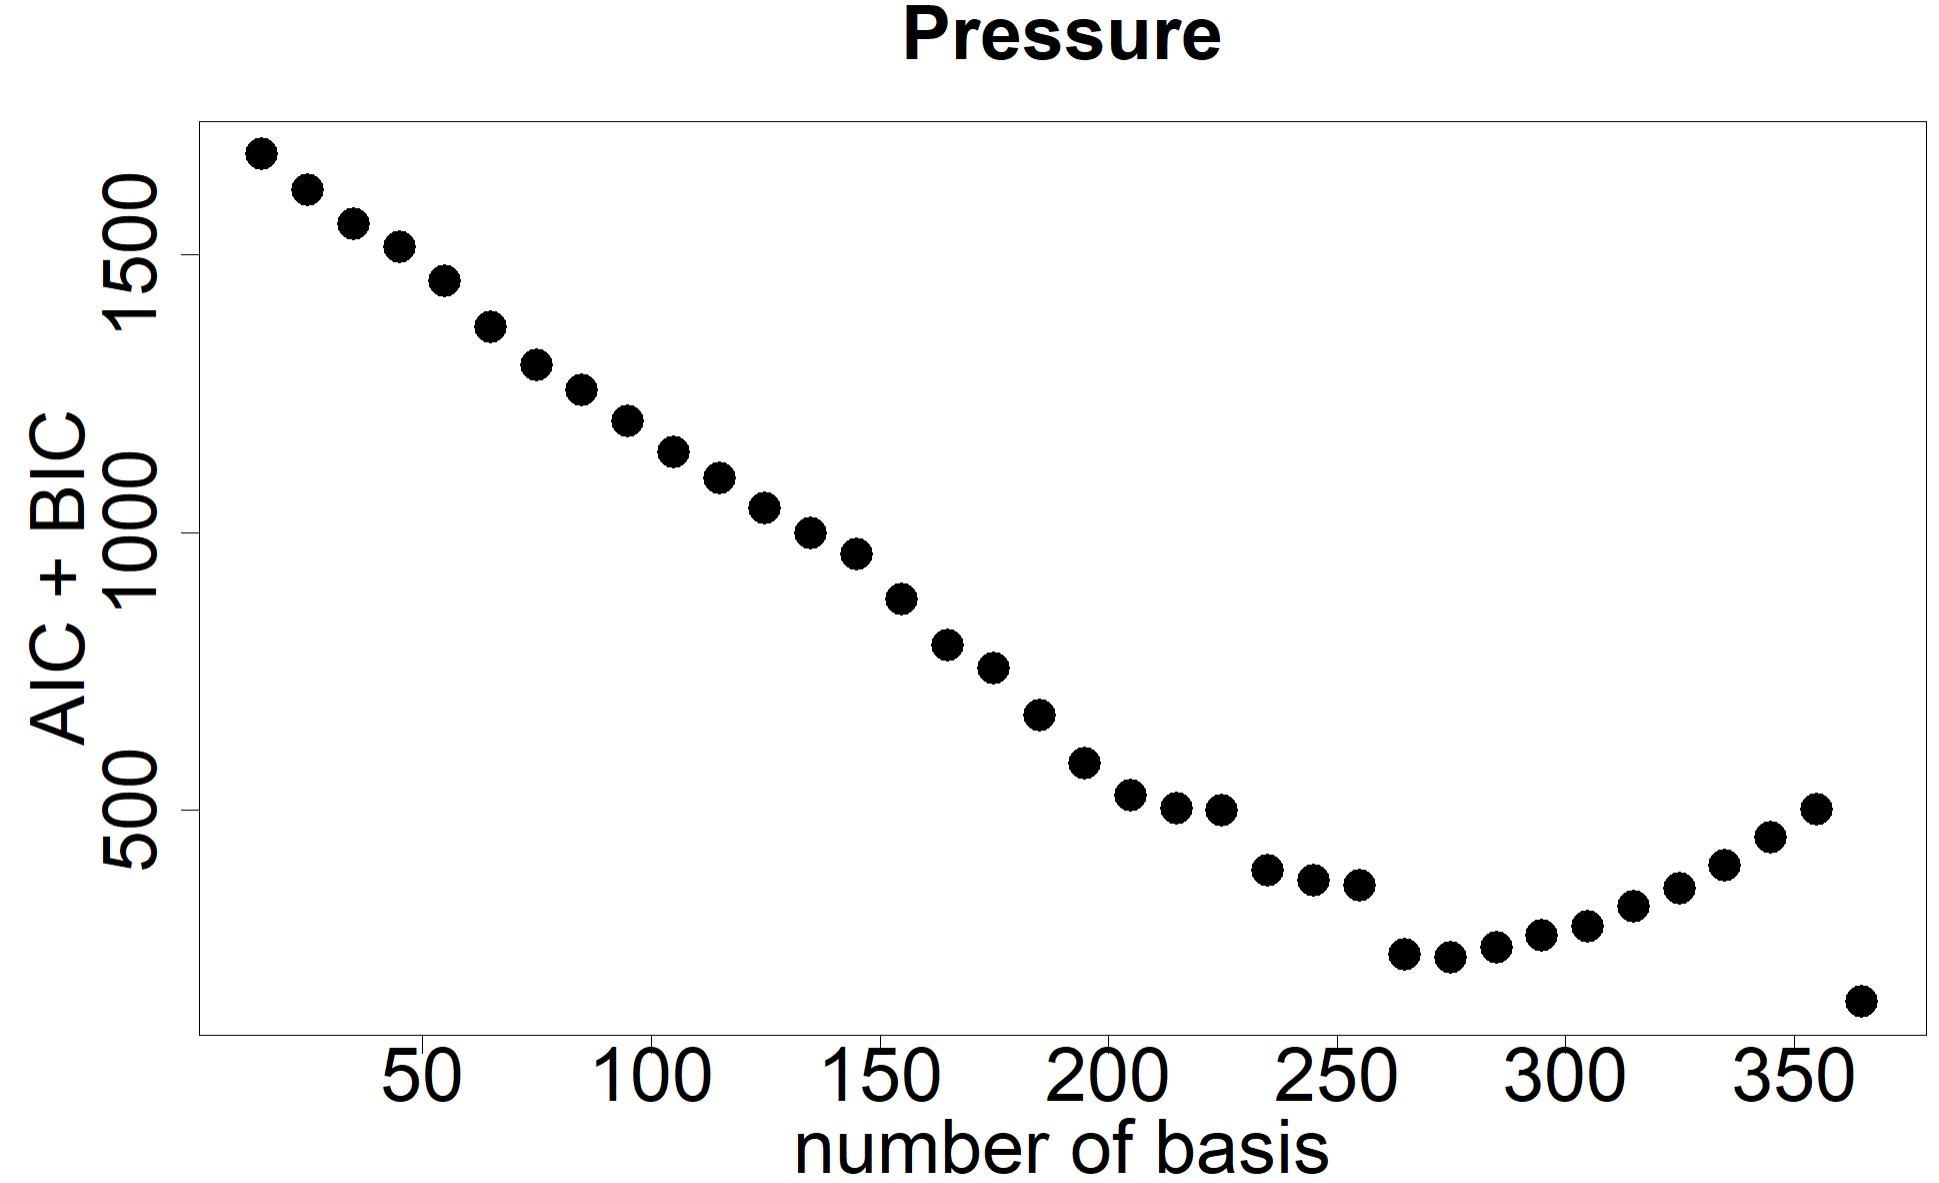
\includegraphics[width=0.47\textwidth]{pressure1}}
\subfigure[]{
\label{Fig.pressure2}
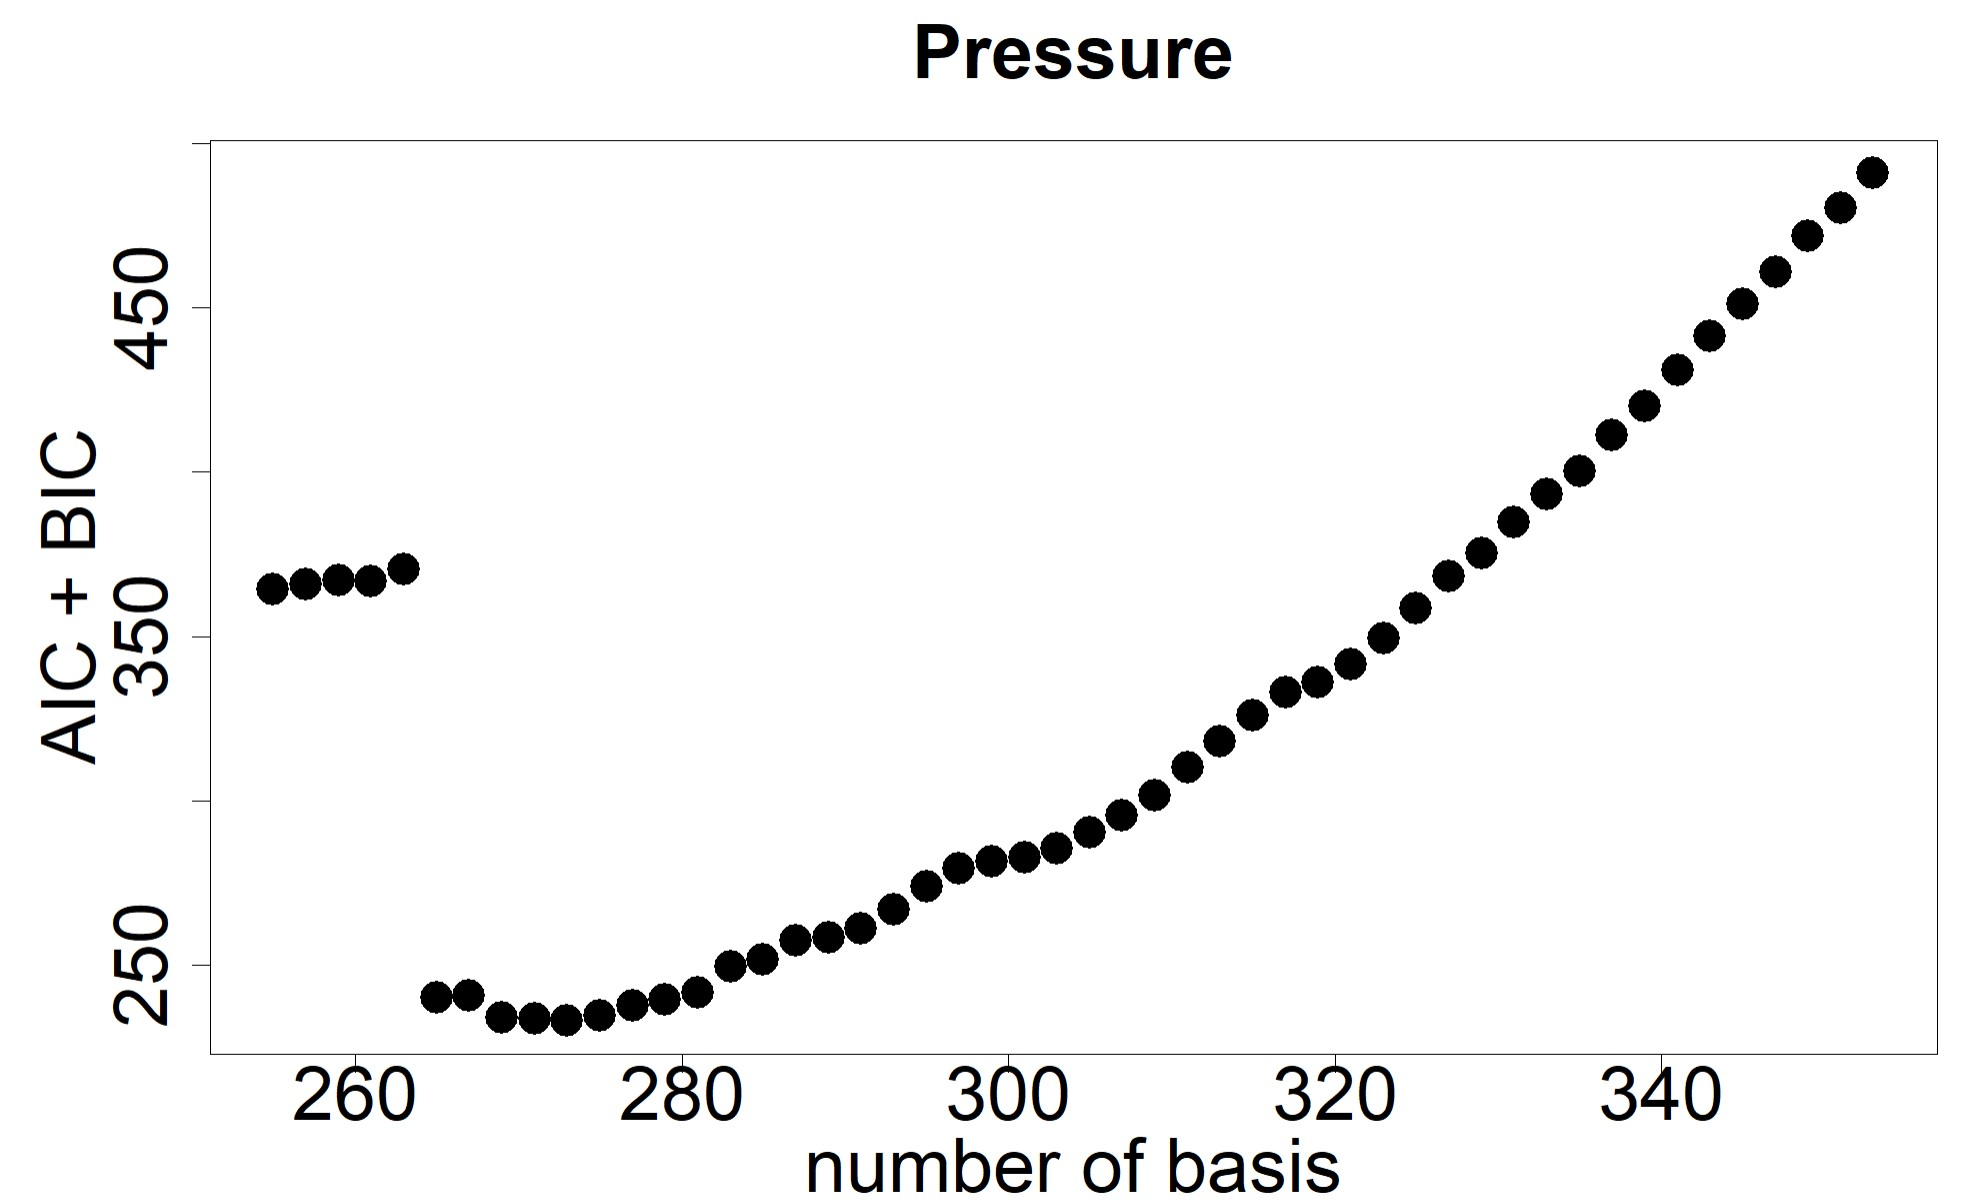
\includegraphics[width=0.47\textwidth]{pressure2}}
\caption{The value of AIC + BIC corresponding to each $\log_{10}(\lambda)$ for Pressure}
%\label{Fig.main}
\end{figure}

\begin{figure}[H]
\centering  %图片全局居中
\subfigure[]{
\label{Fig. sub.1}
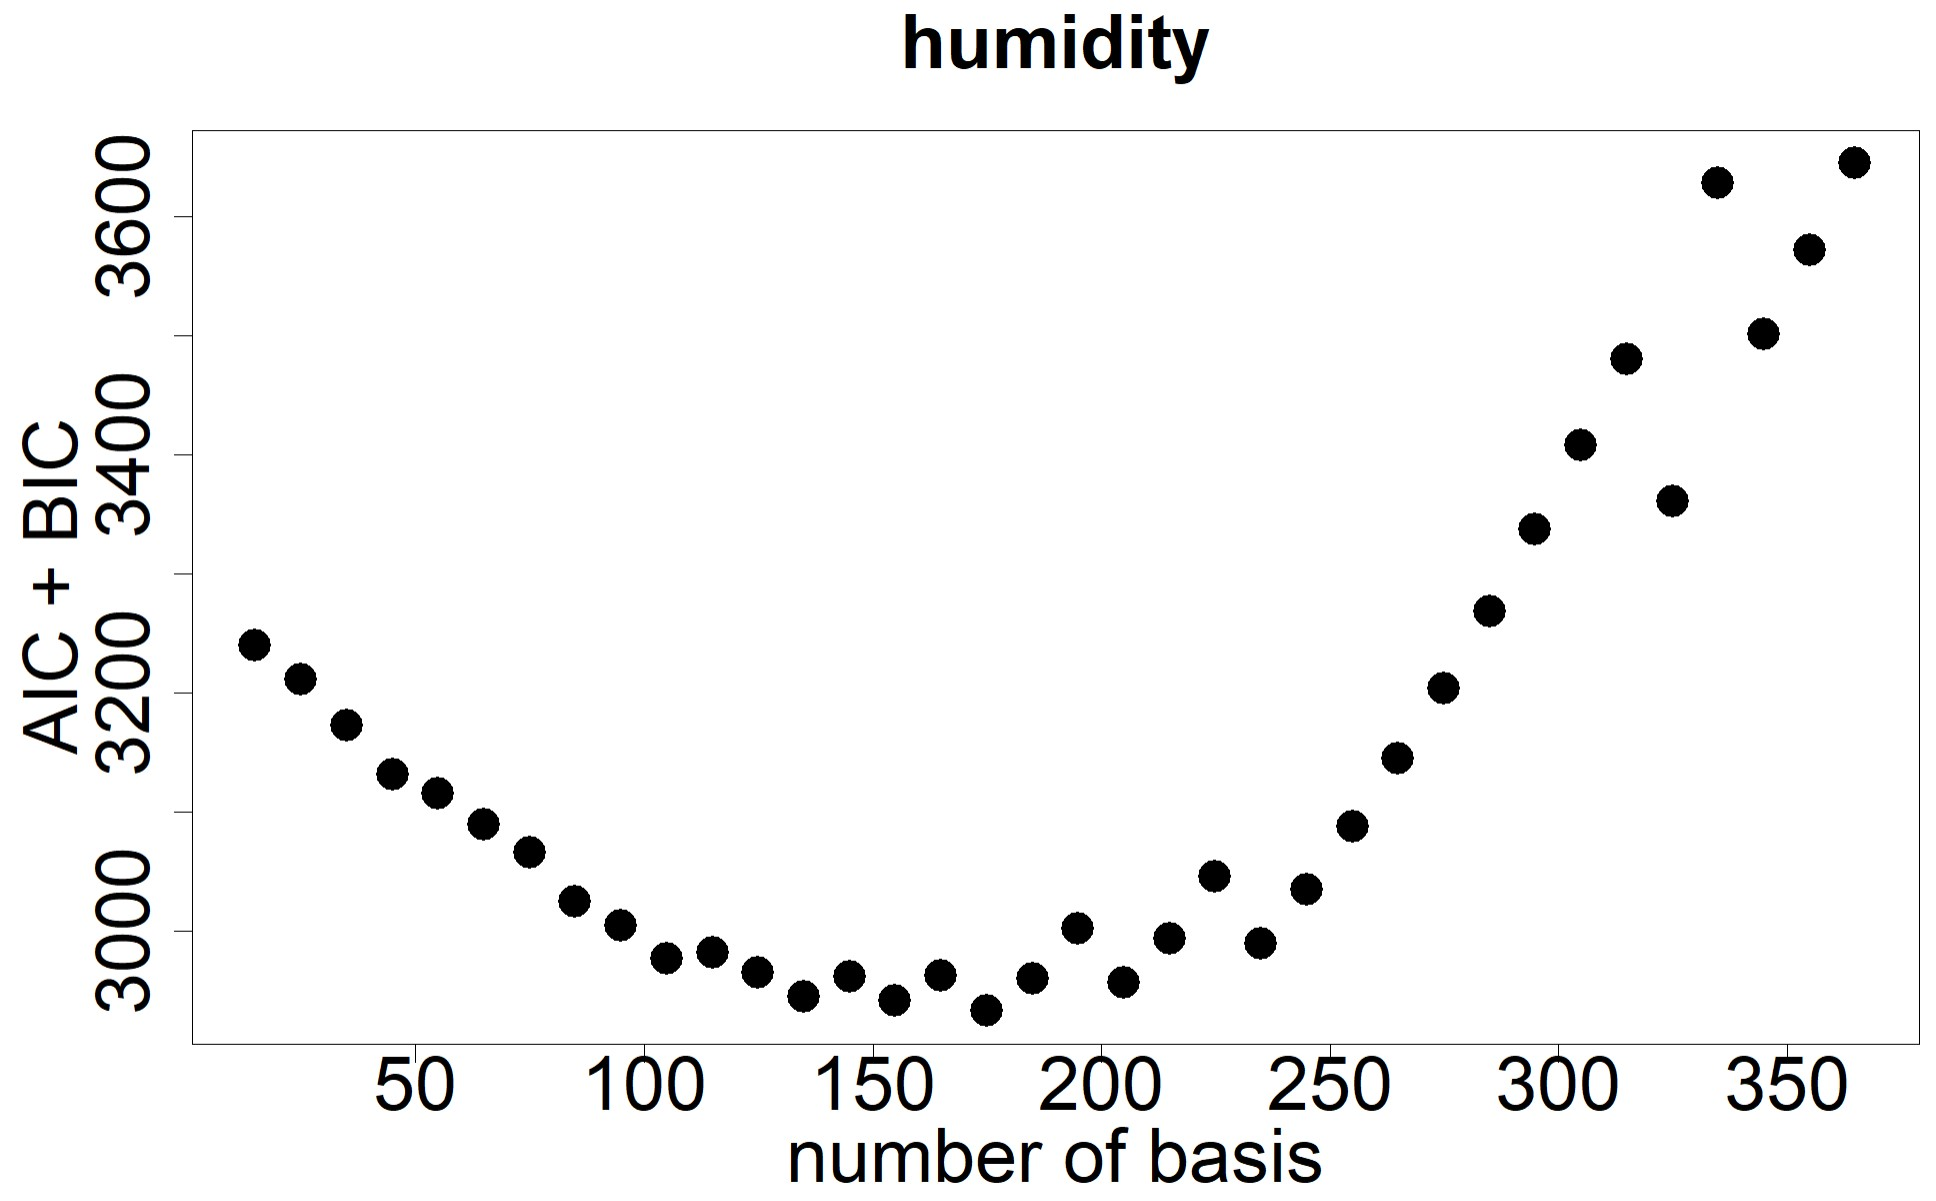
\includegraphics[width=0.47\textwidth]{hum1}}
\subfigure[]{
\label{Fig. sub.2}
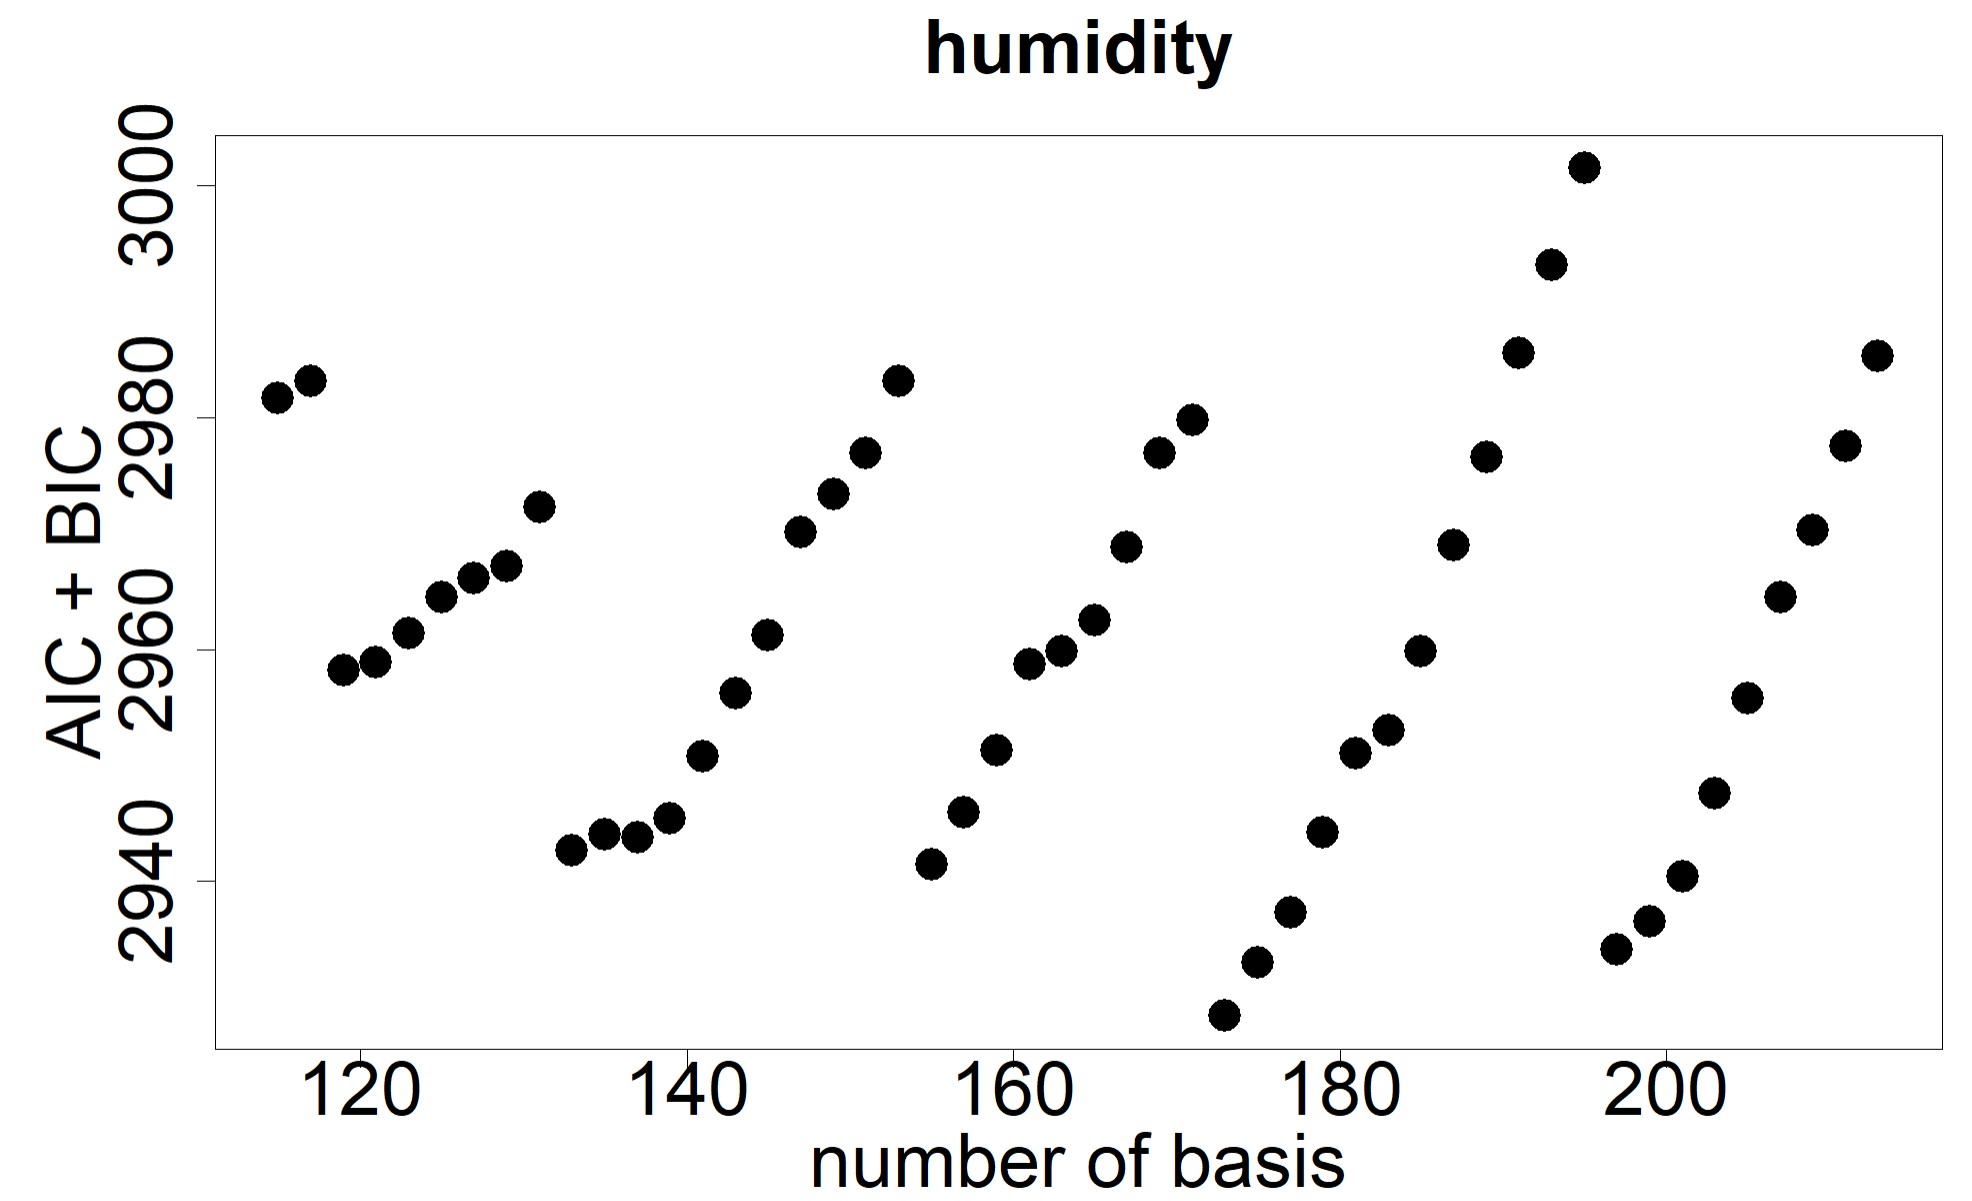
\includegraphics[width=0.47\textwidth]{hum2}}
\caption{The value of AIC + BIC corresponding to each $\log_{10}(\lambda)$ for Humidity}
%\label{Fig.main}
\end{figure}

\begin{figure}[H]
\centering  %图片全局居中
\subfigure[]{
\label{Fig. sub.1}
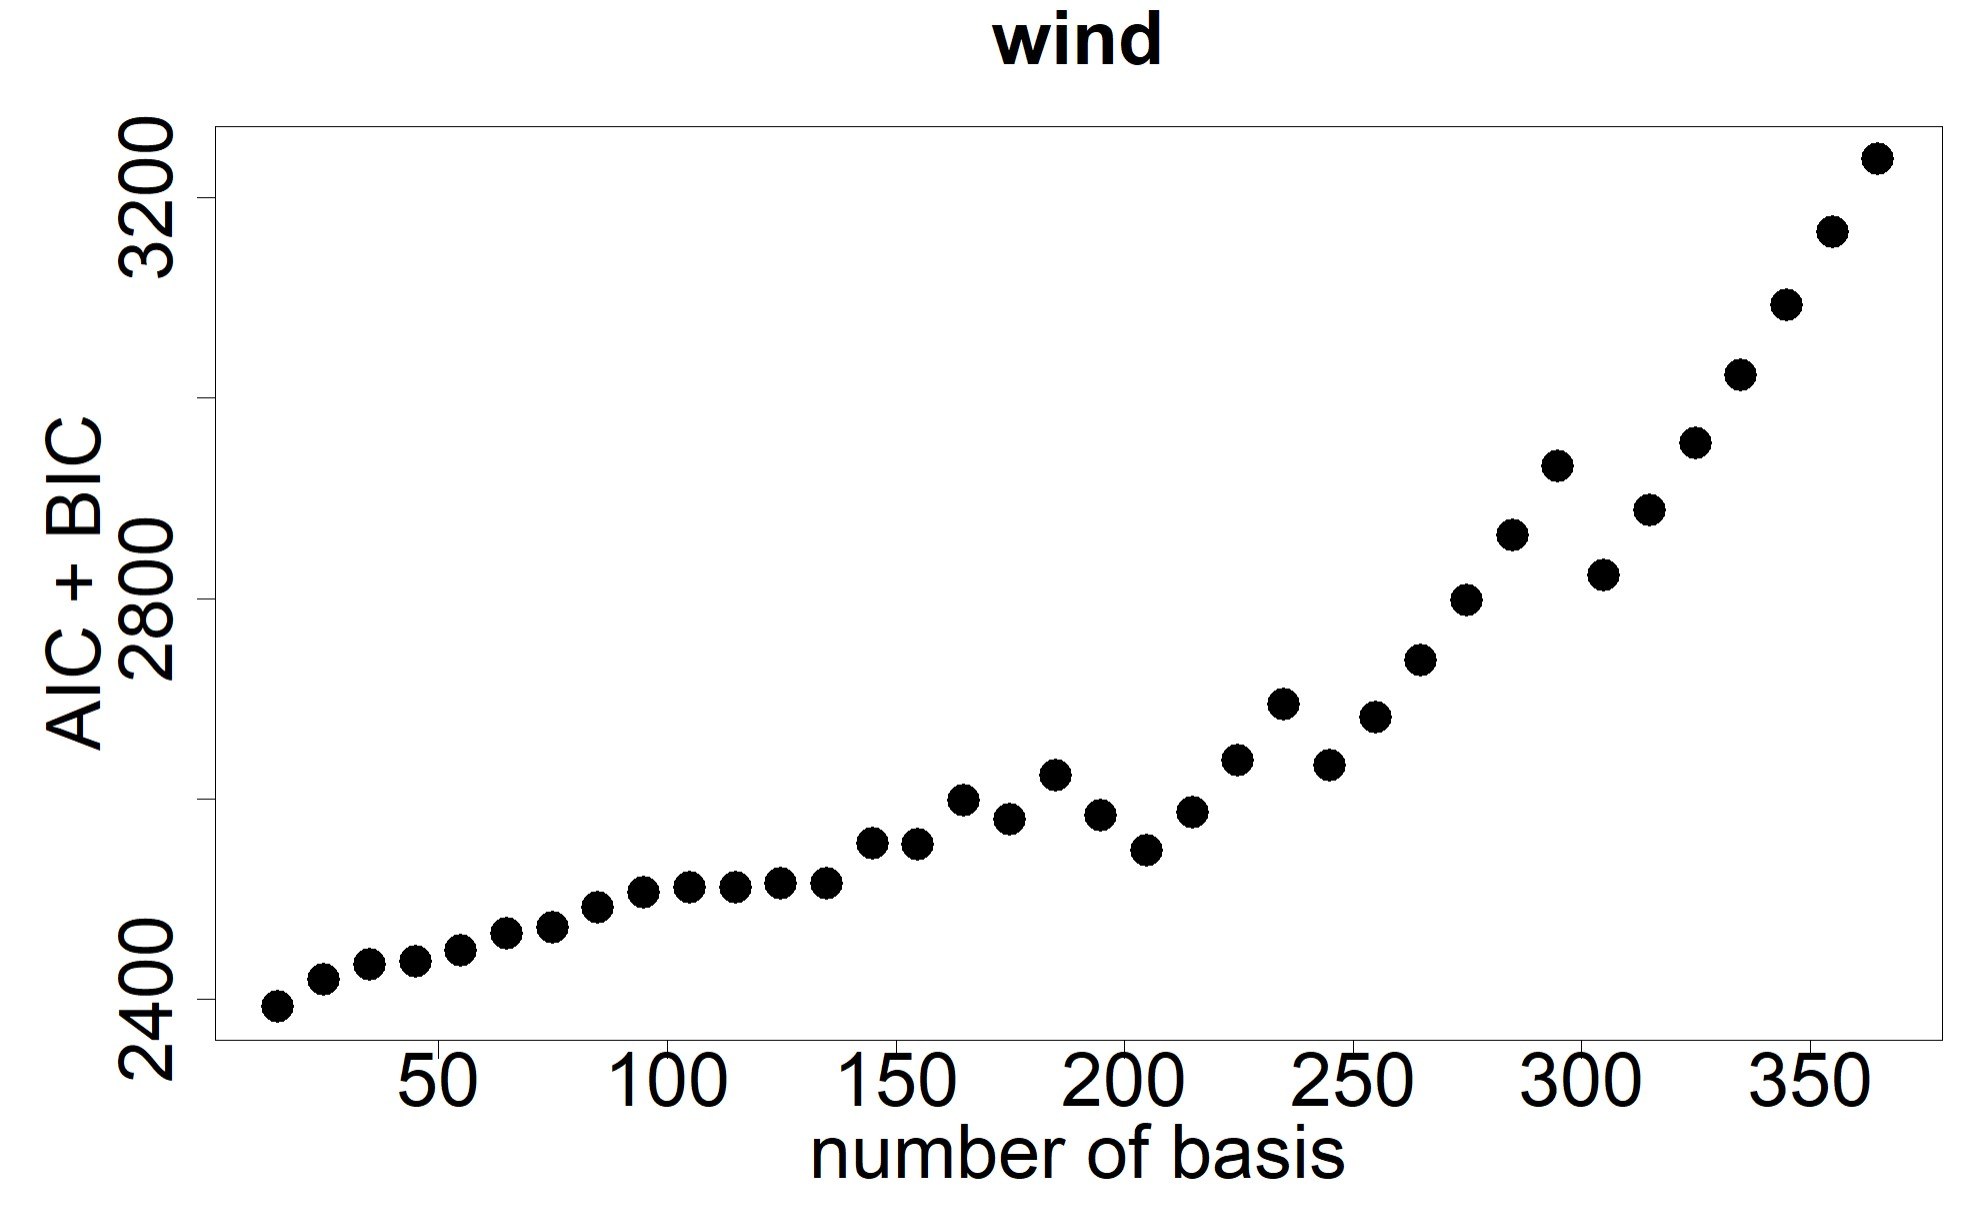
\includegraphics[width=0.47\textwidth]{wind1}}
\subfigure[]{
\label{Fig. sub.2}
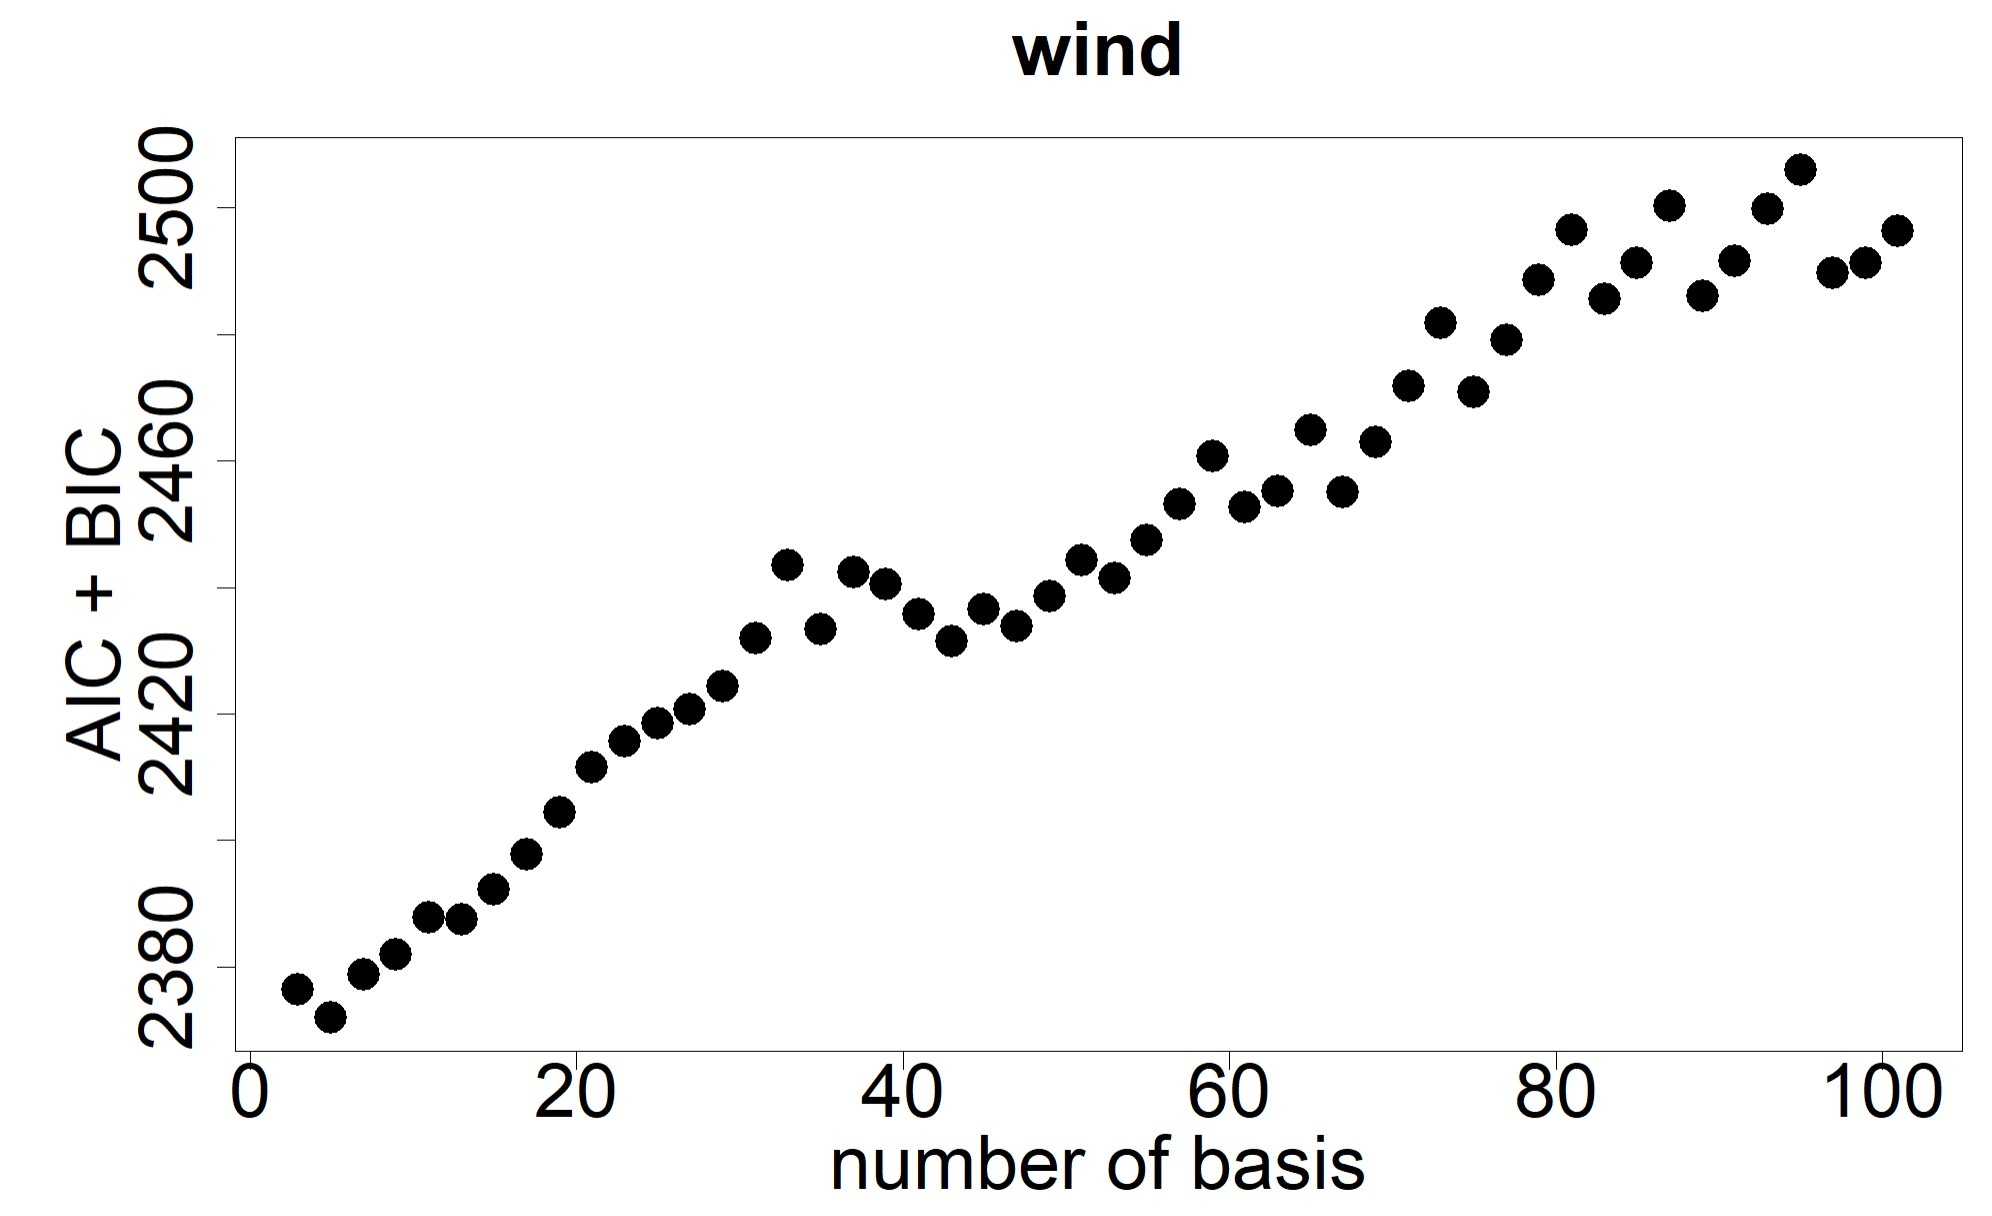
\includegraphics[width=0.47\textwidth]{wind2}}
\caption{The value of AIC + BIC corresponding to each $\log_{10}(\lambda)$ for Wind}
%\label{Fig.main}
\end{figure}

\begin{figure}[H]
\centering  %图片全局居中
\subfigure[]{
\label{Fig. sub.1}
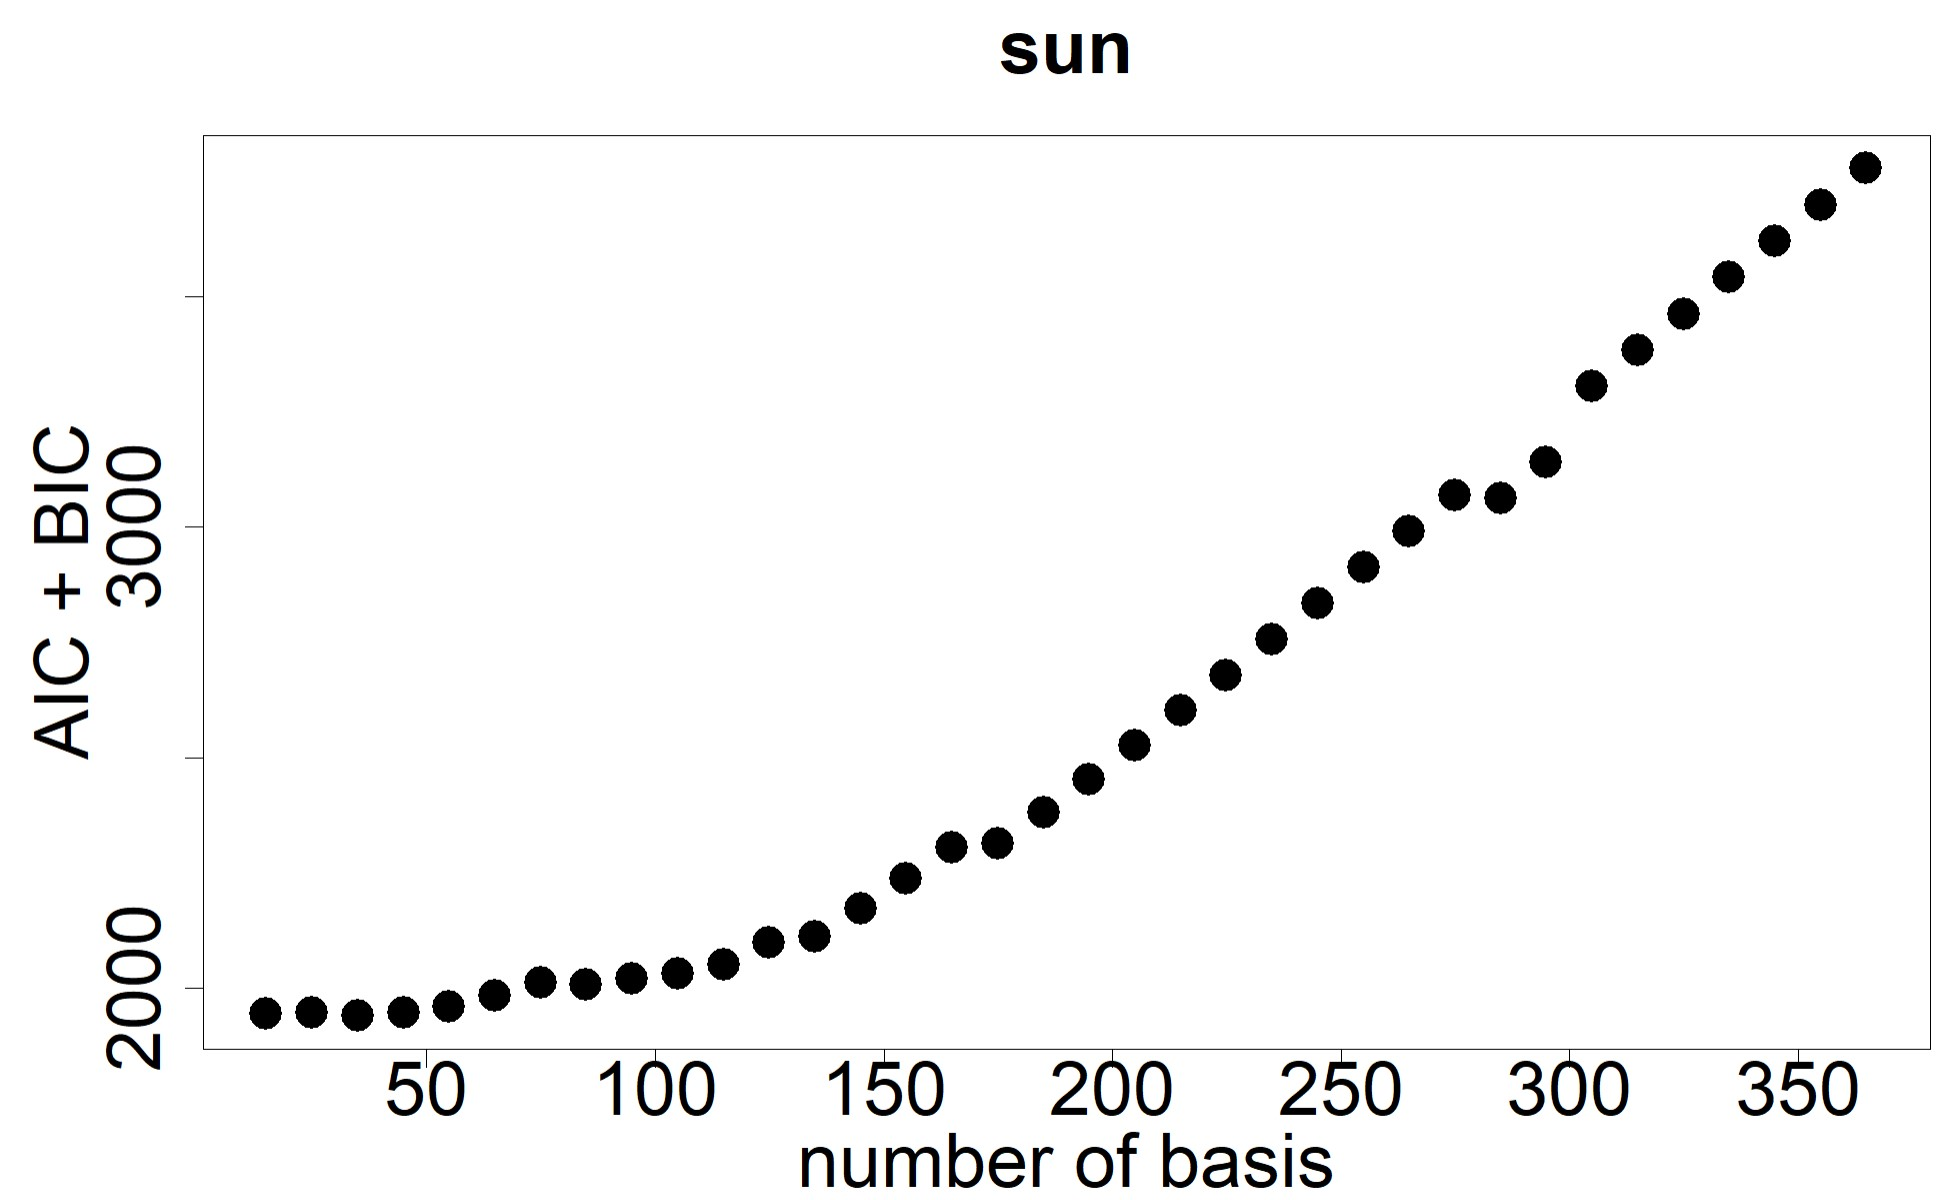
\includegraphics[width=0.47\textwidth]{sun1}}
\subfigure[]{
\label{Fig. sub.2}
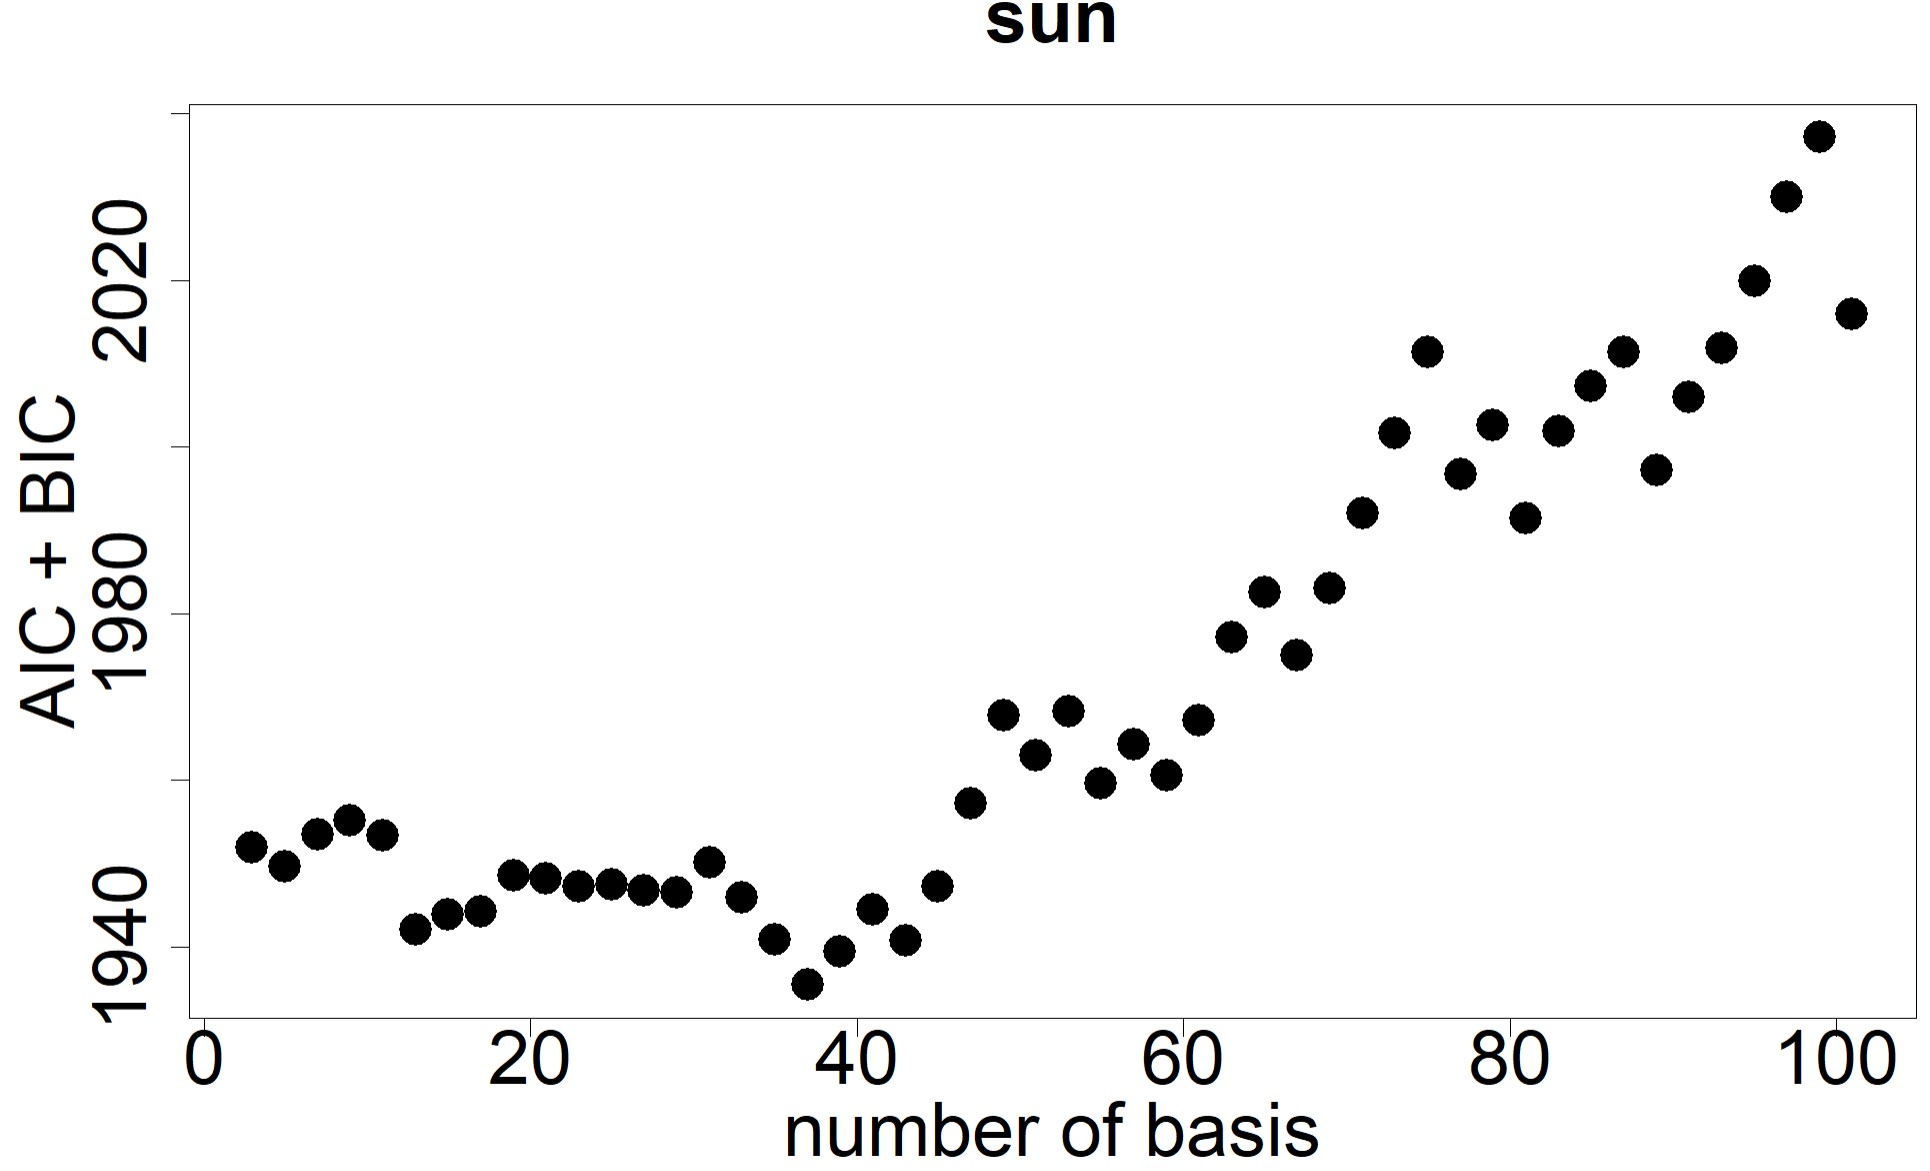
\includegraphics[width=0.47\textwidth]{sun2}}
\caption{The value of AIC + BIC corresponding to each $\log_{10}(\lambda)$ for Sun}
%\label{Fig.main}
\end{figure}

Next, for each covariate, we add a harmonic acceleration linear differential operator $L=\omega^2D+D^3$, where $\omega=2\pi/365$, and get $F(\bm c)=\sum_{j}[y_j-x(t_j)]^2+ \lambda\int[Lx(t)]^2dt$.\\
For choosing the value of $\lambda$, we set a wide range for $\lambda$, we calculate the GCV value for each $\lambda$. Then, we select the $\lambda$ with the minimum GCV value.

The following graphs show the GCV value for each covariate corresponding to $\log_{10}(\lambda)$.

\numberwithin{figure}{section}
\begin{figure}[H] %H为当前位置,!htb为忽略美学标准,htbp为浮动图形
\centering %图片居中
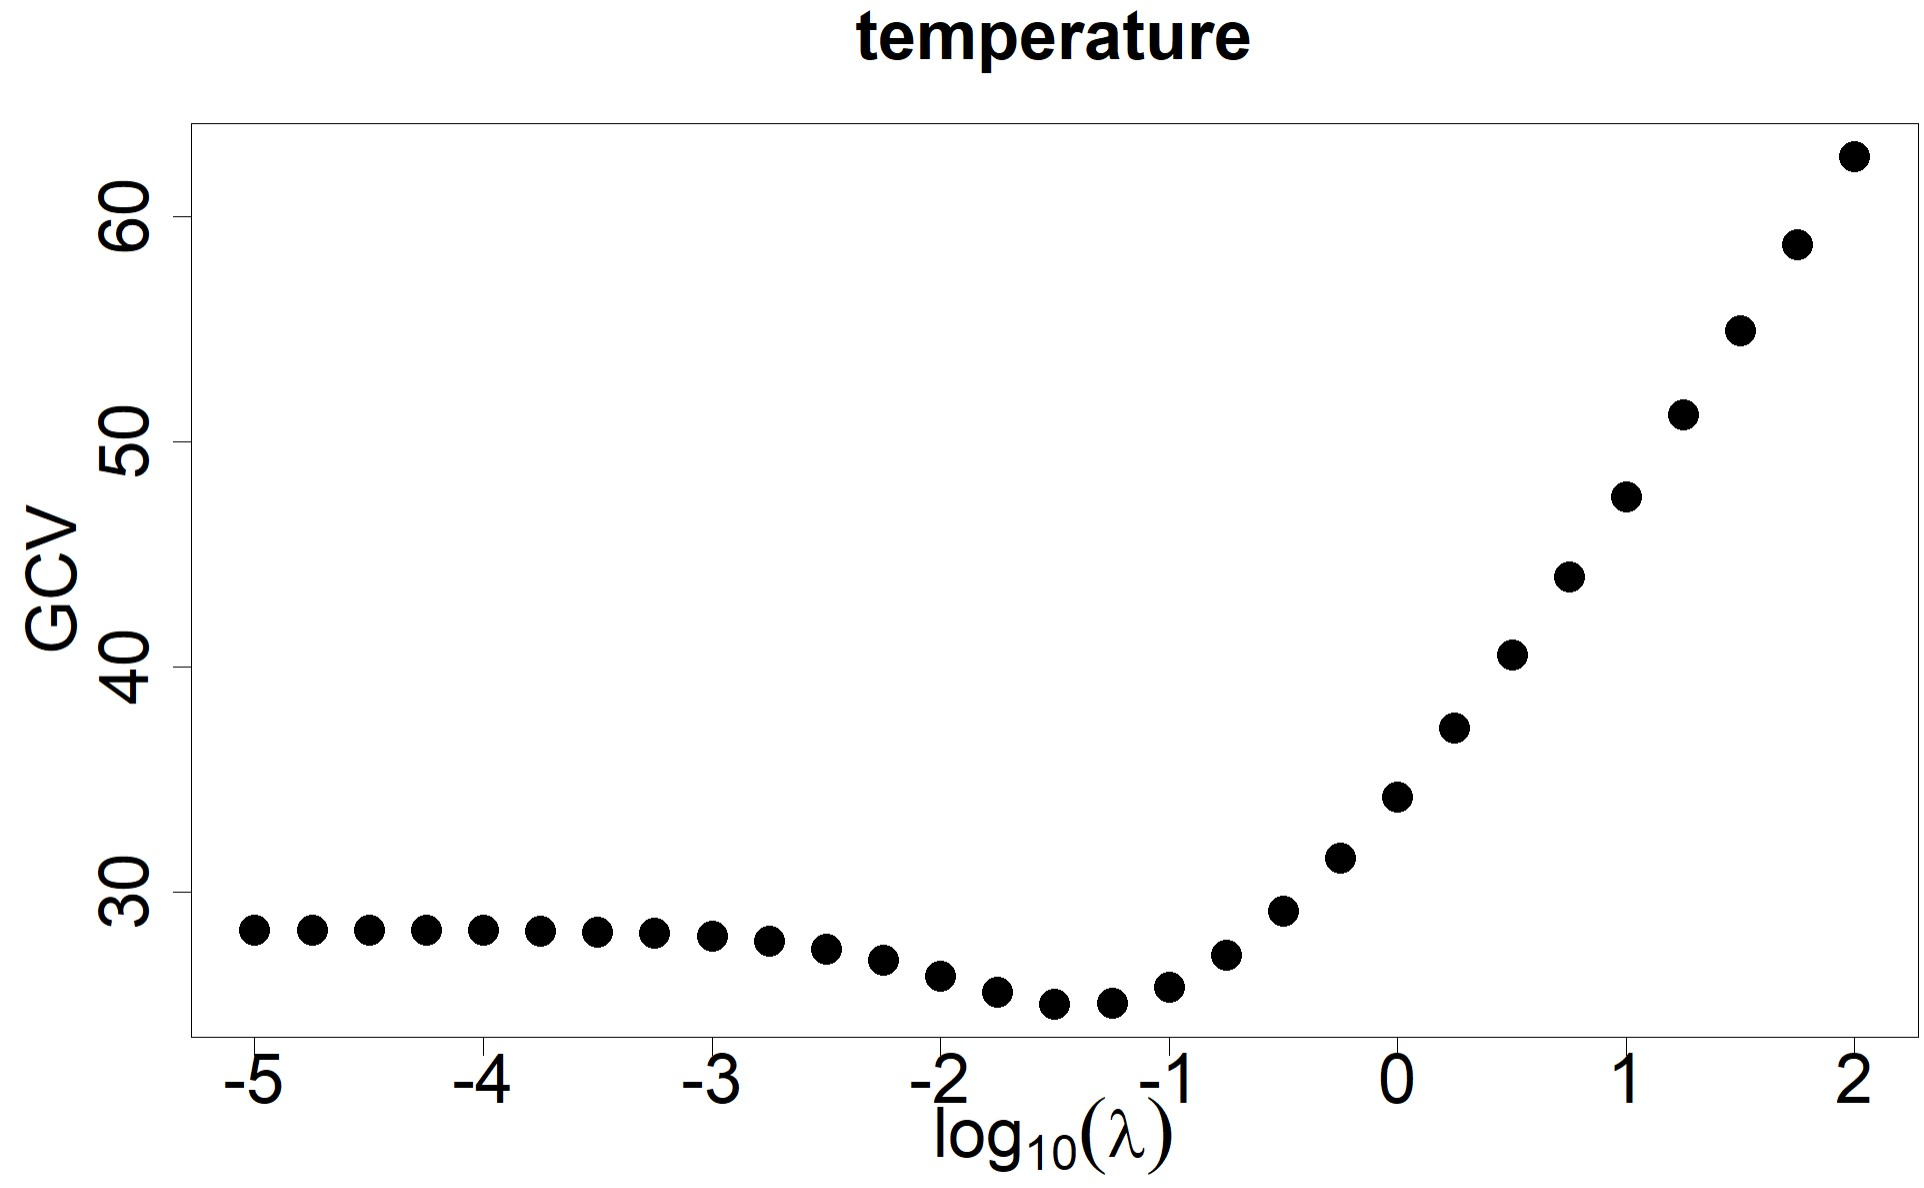
\includegraphics[width=0.73\textwidth]{gcv temp} %插入图片,[]中设置图片大小,{}中是图片文件名
\caption{The GCV value corresponding to each $\log_{10}(\lambda)$ for Temperature} %最终文档中希望显示的图片标题
\label{fig:gcvtemp} %用于文内引用的标签
\end{figure}
%\ref{fig: flowchart}

\numberwithin{figure}{section}
\begin{figure}[H] %H为当前位置,!htb为忽略美学标准,htbp为浮动图形
\centering %图片居中
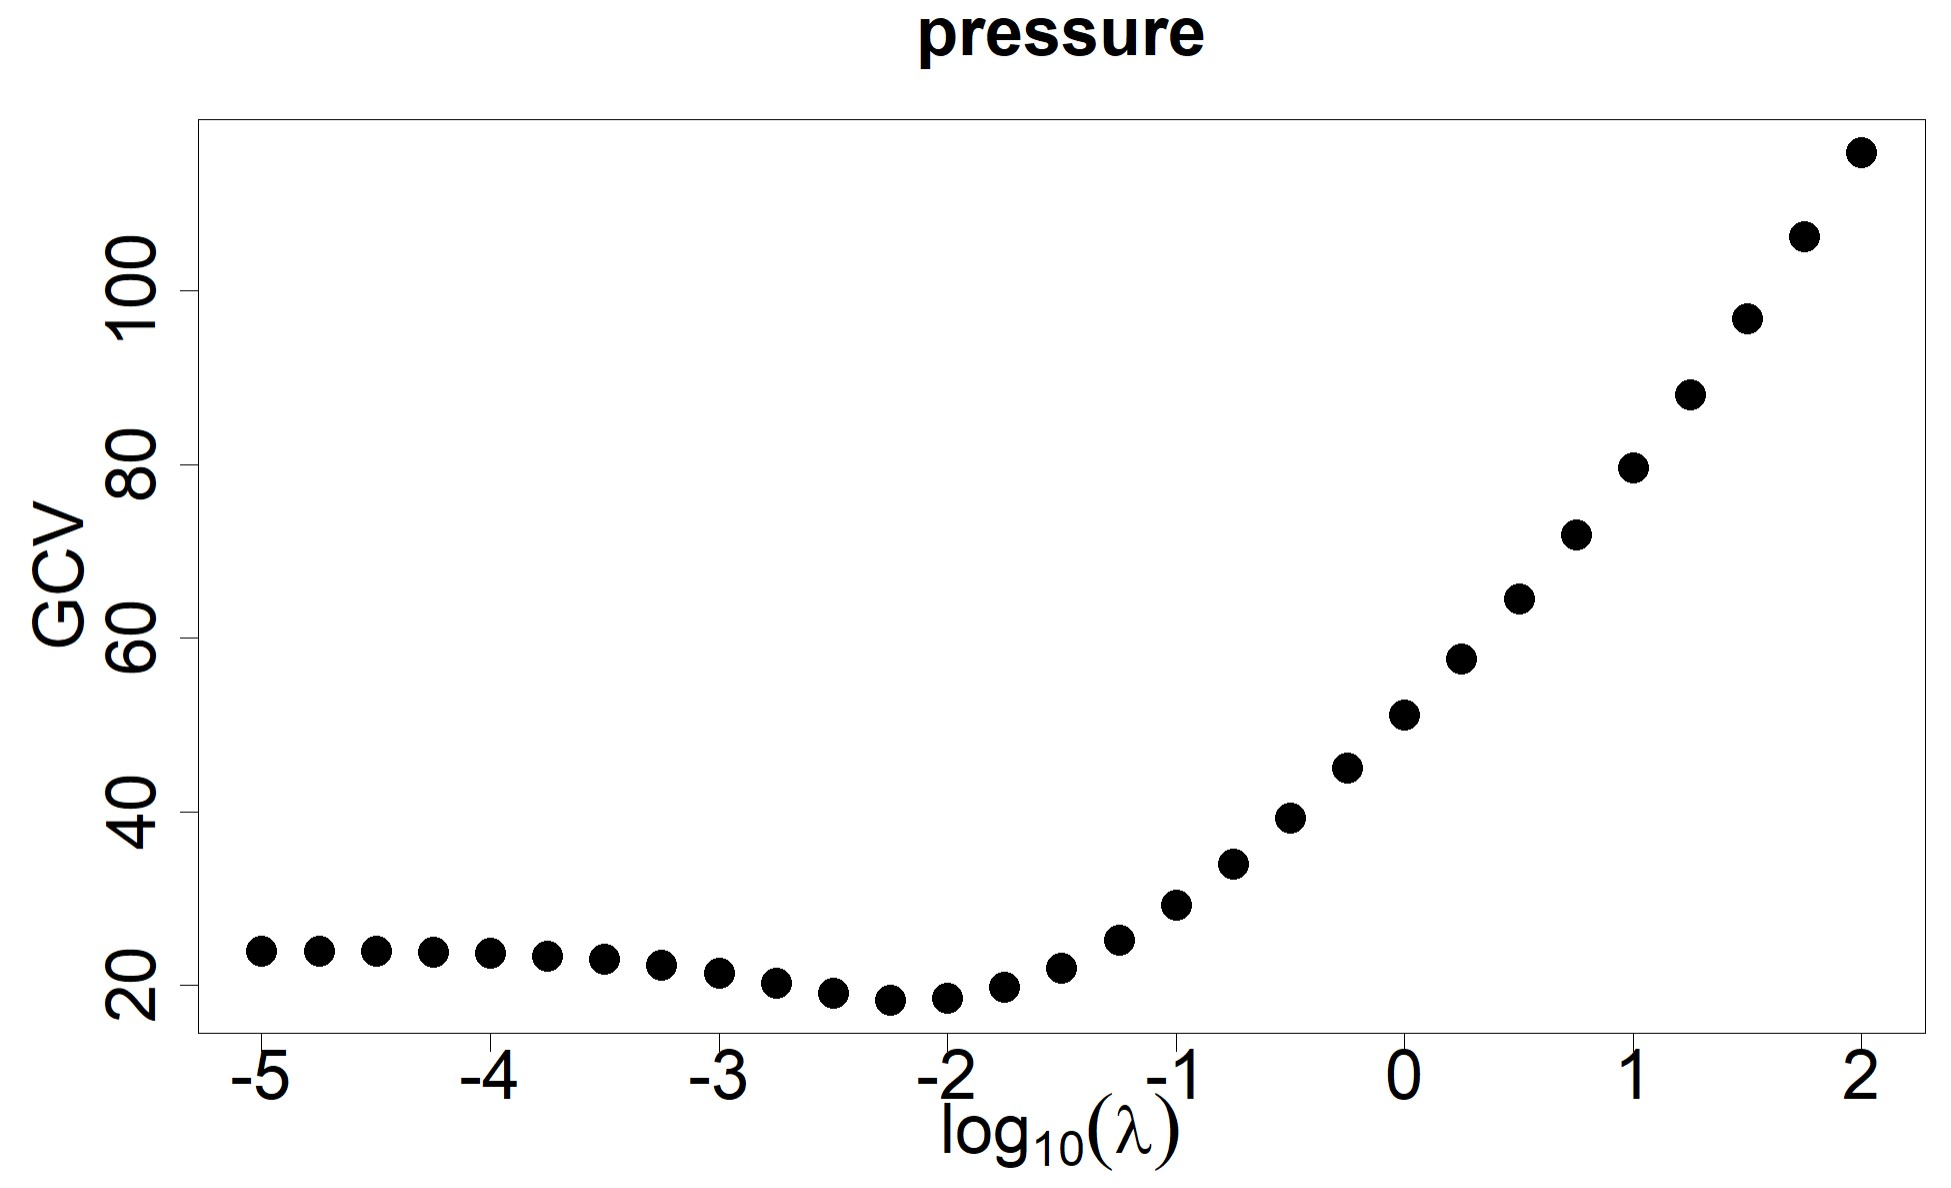
\includegraphics[width=0.73\textwidth]{gcv pressure} %插入图片,[]中设置图片大小,{}中是图片文件名
\caption{The GCV value corresponding to each $\log_{10}(\lambda)$ for Pressure} %最终文档中希望显示的图片标题
\label{fig: gcvpressure} %用于文内引用的标签
\end{figure}
%\ref{fig: flowchart}

\numberwithin{figure}{section}
\begin{figure}[H] %H为当前位置,!htb为忽略美学标准,htbp为浮动图形
\centering %图片居中
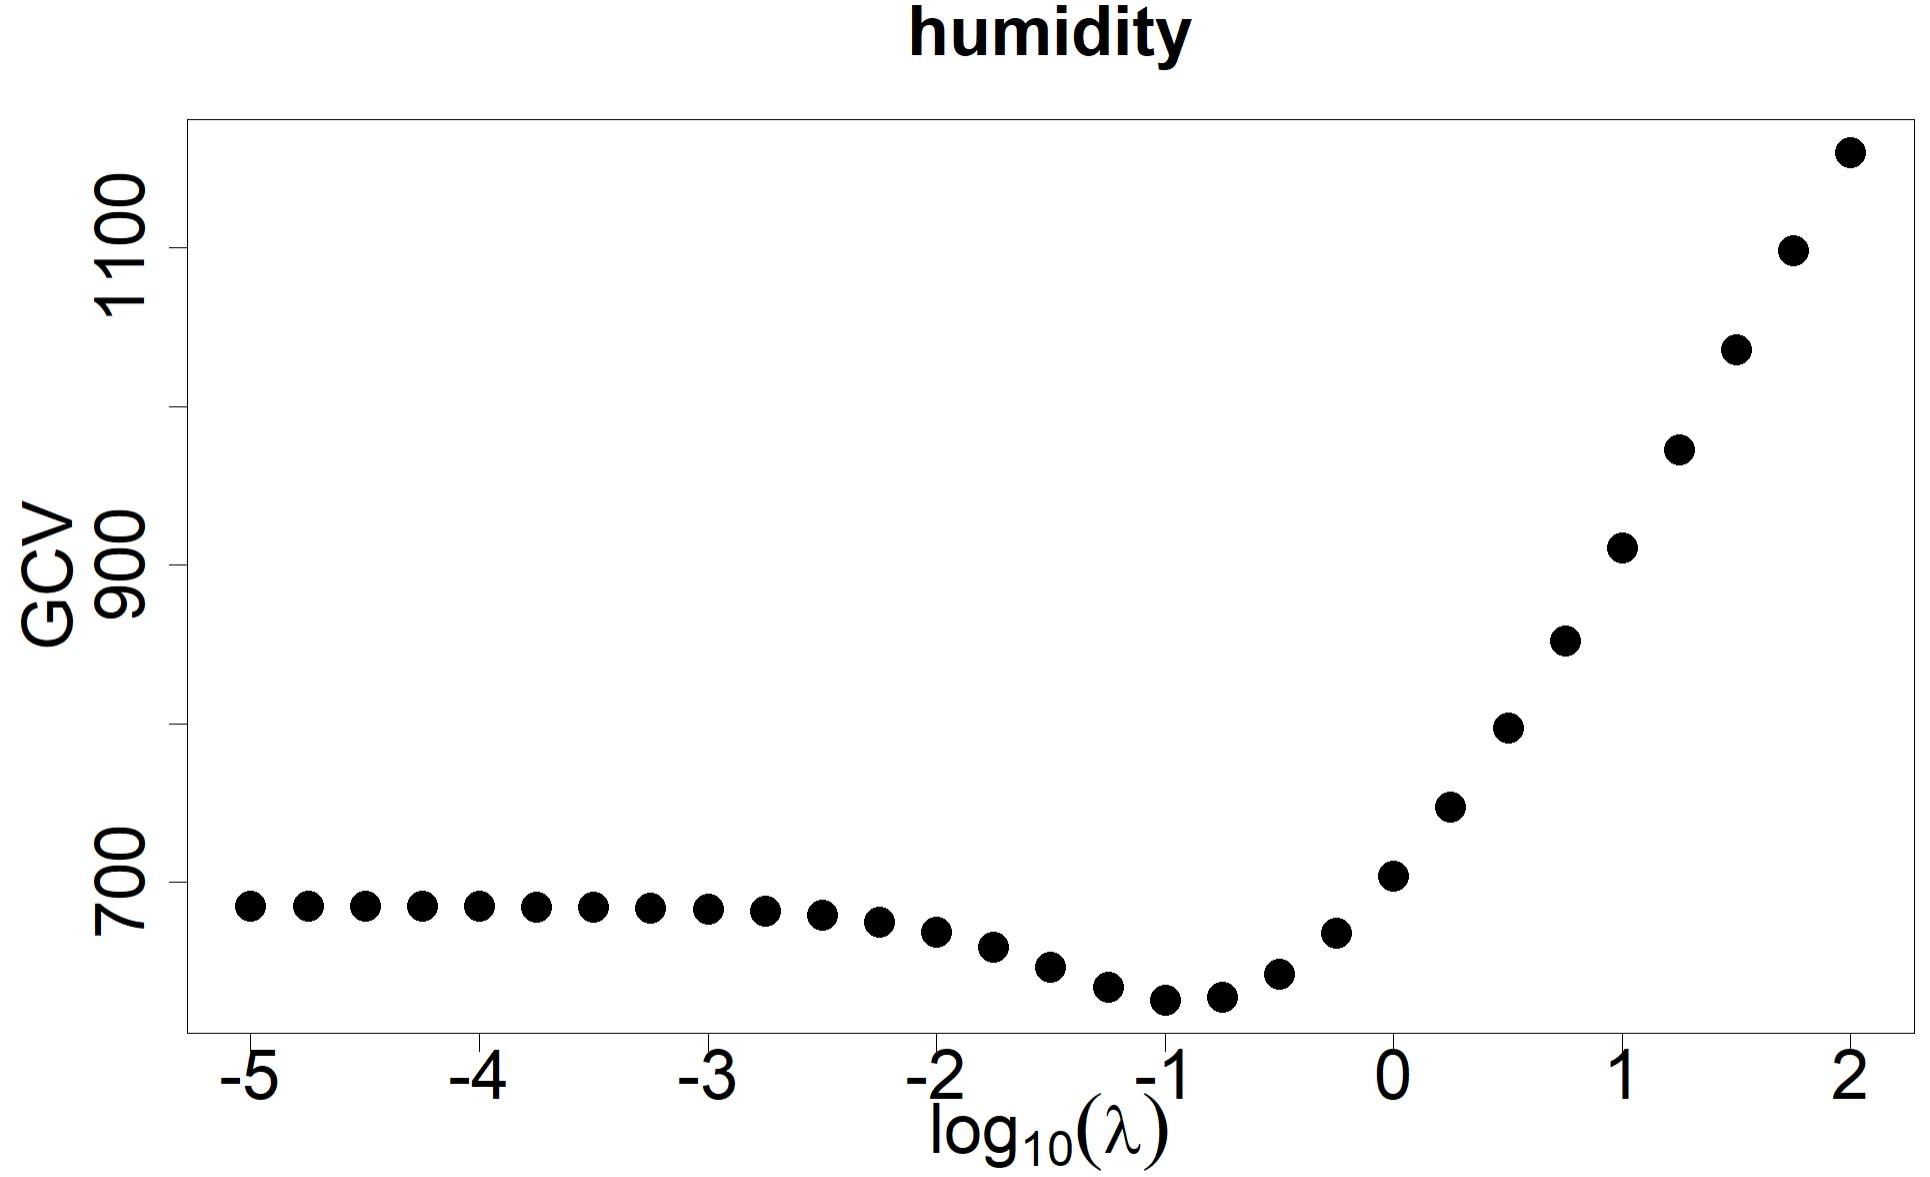
\includegraphics[width=0.73\textwidth]{gcv hum} %插入图片,[]中设置图片大小,{}中是图片文件名
\caption{The GCV value corresponding to each $\log_{10}(\lambda)$ for Humidity} %最终文档中希望显示的图片标题
\label{fig: gcvhum} %用于文内引用的标签
\end{figure}
%\ref{fig: flowchart}

\numberwithin{figure}{section}
\begin{figure}[H] %H为当前位置,!htb为忽略美学标准,htbp为浮动图形
\centering %图片居中
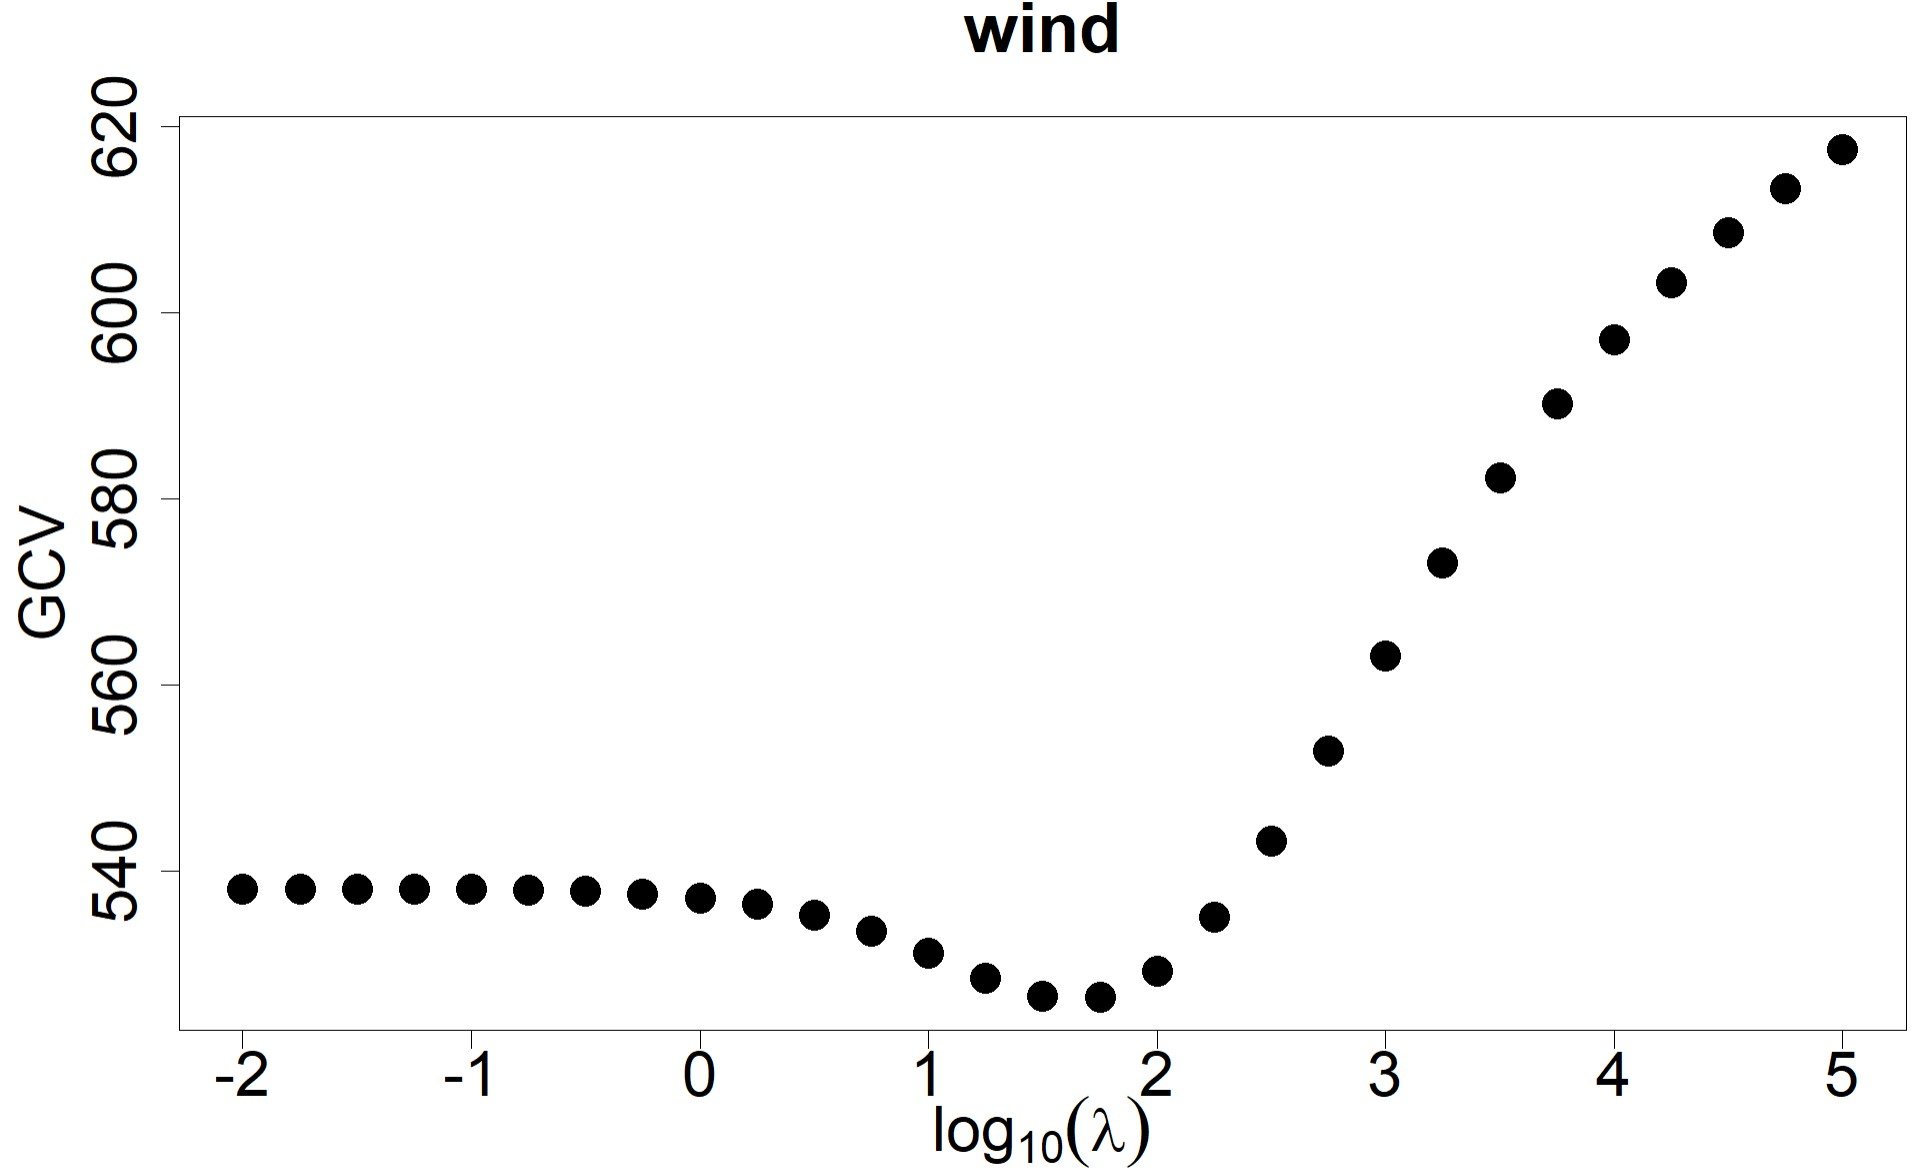
\includegraphics[width=0.73\textwidth]{gcv wind} %插入图片,[]中设置图片大小,{}中是图片文件名
\caption{The GCV value corresponding to each $\log_{10}(\lambda)$ for Wind} %最终文档中希望显示的图片标题
\label{fig: gcvwind} %用于文内引用的标签
\end{figure}
%\ref{fig: flowchart}

\numberwithin{figure}{section}
\begin{figure}[H] %H为当前位置,!htb为忽略美学标准,htbp为浮动图形
\centering %图片居中
\includegraphics[width=0.73\textwidth]{gcv Sun} %插入图片,[]中设置图片大小,{}中是图片文件名
\caption{The GCV value corresponding to each $\log_{10}(\lambda)$ for Sun} %最终文档中希望显示的图片标题
\label{fig:gcvsun} %用于文内引用的标签
\end{figure}
%\ref{fig: flowchart}
Eventually, when we get the number of basis functions and $\lambda$ for each covariate, we use the function $" smooth.basis"$ in package $"fda"$ in R to get the functional data object. 

\subsection{Functional Linear Model with the Original Five Covariates to Scalar Response}
In this part, we fit yearly average precipitation $y$ (a scalar response) by using all the other 5 covariates (5 functional covariates). \\
$$y_i=\alpha_0+\ \sum_{j=1}^{5}\int{x_{ij}\left(t\right)\beta_j\left(t\right)dt}+\epsilon_i,$$
where $y_i$ is the average precipitation for each year and the coefficient (weight) functions:
$$\beta\left(t\right)=\ \sum_{k}^{K}{c_k\phi_k\left(t\right)}=\bm{c}^\prime\bm{\phi}\left(t\right).$$
In the beginning, the data set was divided into a training set and a test set randomly, the training set contains the data within 20 years while the test set involves data within the rest 4 years.

Additionally, 5-fold cross-validation is used on the training set to select the number of basis functions for each $\beta_j(t),j = 1,\dots,5.$ The number of basis functions corresponding to the minimum mean squared prediction error is used in the model,
$$MSPE=\ \sum_{b=1}^{B}\sum_{l\in S_b}^{N}{\frac{\left({\hat{y}}^{\left(-b\right)}-y_l\right)^2}{N}\ },$$
where $S_b$ is the $b$-th partition of the training data set and ${\hat{y}}^{(-b)},l\in S_b,$ is the prediction in the set. 

After confirming the number of basis functions for each $\beta_j(t), j =1,\dots,5$, we plug them into the whole training set to get a functional linear model, and at last, test the model with the test set. $R^2$ for the test set is an evaluation of the fit of the model:\\
$$R^2=1-\ \sum_{l=1}^{N}{\left(y_l-{\hat{y}}_l\right)^2/\sum_{l=1}^{N}\left(y_l-\bar{y}\right)^2}.$$
Notice that from Section 2, we can estimate coefficients $\hat{\bm{b}}$ by $\hat{\bm{b}}=\left(\bm{Z}^\prime\bm{Z}\right)^{-1}\bm{Z}^\prime\bm{y}$, and 

$$\mathbf{Z}=\left[\begin{matrix}{1}&\int{x_{11}\left(t\right)\mathbf{\Phi}_{1}\left(t\right)dt}\ \ \ \ \ \ldots&\int{x_{1q}\left(t\right)\mathbf{\Phi}_{5}\left(t\right)dt}\\\vdots&\ddots\ &\vdots\\{1}&\int{x_{n1}\left(t\right)\mathbf{\Phi}_{1}\left(t\right)dt\ }\ \ \ \ \ldots&\int{x_{nq}\left(t\right)\mathbf{\Phi}_{5}\left(t\right)dt}\\\end{matrix}\right].$$

However, if we simply use the FLM model without a penalty term, the matrix $\bm{Z}^\prime\bm{Z} $will not be invertible if we have more than 3 basis functions for each $ \beta_j\left(t\right),\ j\ =\ 1,\dots,5, $ thus we cannot get $\hat{\bm{b}}=\left(\bm{Z}^\prime\bm{Z}\right)^{-1}\bm{Z}^\prime\bm{y}.$ The reason why this issue occurs is that we only got 16 functional data objects in our training set, while there are 5 covariates. If we let $\beta_j\left(t\right)\ $for each covariate to be spanned by more than 3 basis functions, the matrix $\bm{Z}^\prime\bm{Z}$ will be a singular matrix. And of course, the performance for this FLM model is bad since 3 basis functions are not enough for each $\beta_j\left(t\right)$.

To solve this problem, we add a penalty term while solving the least square problem. Thus, the estimator by least square with ridge penalty as shown in Section 2 is given by: 
$$\hat{\bm b}=\left(\bm{Z}^\prime\bm{Z}+\bm{R}(\lambda)\right)^{-1}\bm{Z}^\prime\bm{y},$$
where ridge penalty matrix $R(\lambda)$ is 
$$R=\left[\begin{matrix}1&\ldots&\ldots&\ldots\\0&\lambda_1R_1&\ldots&0\\\vdots&\vdots&\ddots&\vdots\\0&0&\ldots&\lambda_5R_5\\\end{matrix}\right].$$
Eventually, this newly calculated $\hat{\bm b}$ is used for the current yearly average precipitation regression.

Similarly, we construct a prediction model aimed to get the yearly average precipitation for the next year. The only thing different from the previous procedure is adding the yearly average precipitation in the current year as a new scalar covariate. So, our corresponding formula, matrix $Z$ and $R$ changed into the following forms,
$$y_i=\alpha_0+{\alpha}_{1}{z}_{i}+ \sum_{j=1}^{5}\int{x_{ij}\left(t\right)\beta_j\left(t\right)dt}+\epsilon_i,$$
$$\mathbf{Z}=\left[\begin{matrix}{\ {1}\ \ \ {z}}_{1}&\int{x_{11}\left(t\right)\mathbf{\Phi}_\mathbf{1}\left(t\right)dt}\ \ \ \ \ \ldots&\int{x_{1q}\left(t\right)\mathbf{\Phi}_\mathbf{5}\left(t\right)dt}\\\vdots&\ddots\ &\vdots\\\ \ {1}\ \ \ {z}_{n}&\int{x_{n1}\left(t\right)\mathbf{\Phi}_\mathbf{1}\left(t\right)dt\ }\ \ \ \ \ldots&\int{x_{nq}\left(t\right)\mathbf{\Phi}_\mathbf{5}\left(t\right)dt}\\\end{matrix}\right],$$
$$
R =\left[\begin{matrix}I_{2\times2}&\ldots&\ldots&\ldots\\0&\lambda_1R_1&\ldots&0\\\vdots&\vdots&\ddots&\vdots\\0&0&\ldots&\lambda_5R_5\\\end{matrix}\right].
$$
After the same calculation, we can get $\hat{\bm b}$ and make the prediction. The reason why we do this additional prediction is stated in Section 3.6.

\subsection{Functional Score Regression with Three Principal Components to Scalar Response}
The only difference between this section (3.4) to the last section (3.3) is that we use the newly generated 3 principal components to replace the original 5 covariates since it can ease the multicollinearity problem among the covariates.

First of all, we do principal component analysis among the 5 covariates each year. The total variance explained in each year by different PCs is shown in Figure \ref{fig:pcr}. We found that the first 3 principal components for all 24 years can explain around 95$\%$ of the variance, significantly greater than the first two components while only slightly less than the first four components, that’s why we use the scores of those 3 PCs as new covariates. 

\numberwithin{figure}{section}
\begin{figure}[H] %H为当前位置,!htb为忽略美学标准,htbp为浮动图形
\centering %图片居中
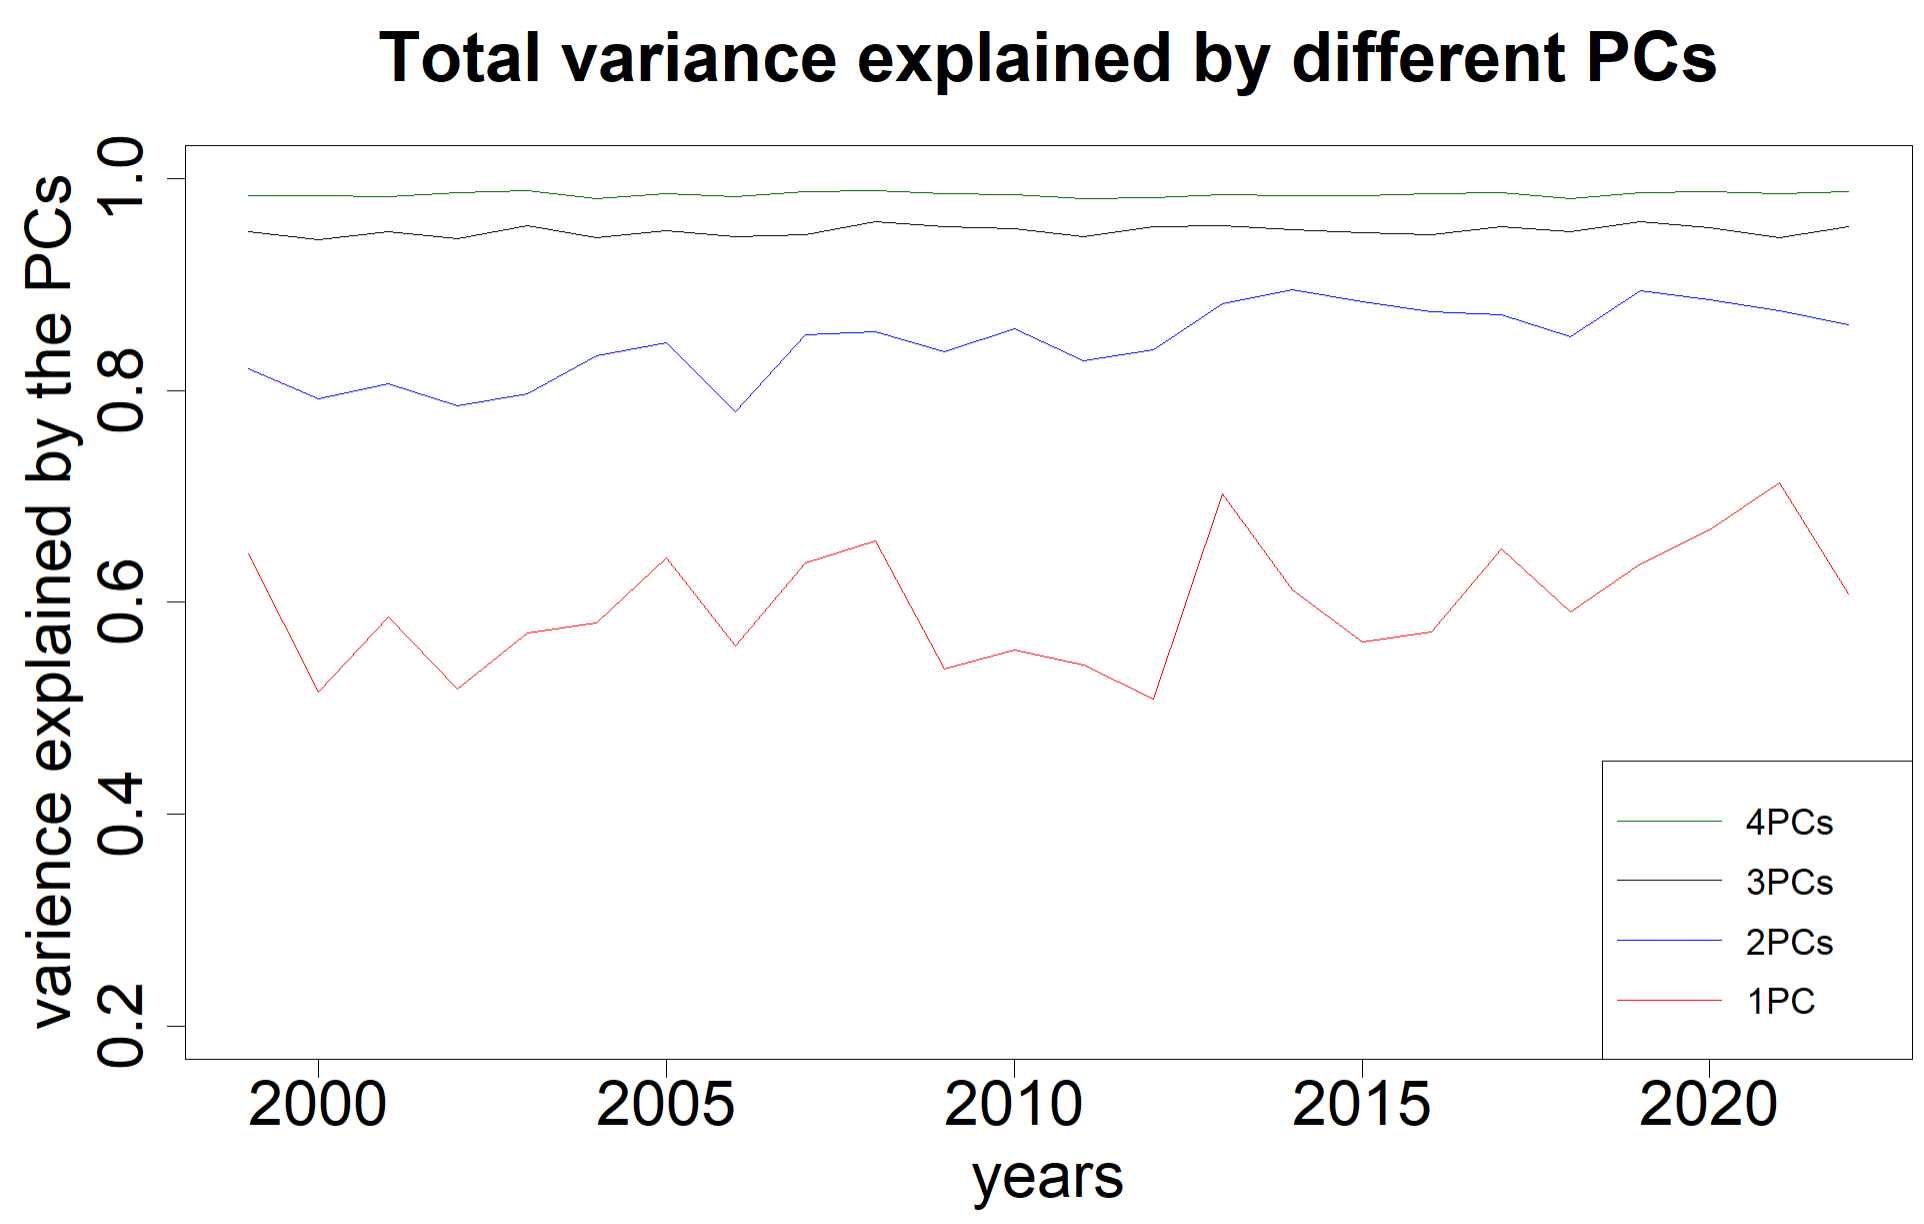
\includegraphics[width=0.8\textwidth]{3PCs.png} %插入图片,[]中设置图片大小,{}中是图片文件名
\caption{Variance explained by the first 4 PCs for all 24 years} %最终文档中希望显示的图片标题
\label{fig:pcr} %用于文内引用的标签
\end{figure}
%\ref{fig: flowchart}
After getting 3 PCs for all 24 years, we smooth the scores of PCs obtaining score functions, and we conduct a penalized FLM with those smoothed data. After doing a regression on the current year, we also perform a prediction for the next year as in Section 3.3.

\subsection{Functional Neural Networks to Scalar Response}
For Functional Neural Networks, we can directly put the smoothed data into the model using package $" fun.fit"$ in R, and select different hyperparameters. In this specific example, we tune the model with different numbers of bases for the functional coefficients, different activation functions like sigmoid, ReLU, LeakyReLU, tanh, and so on, different numbers of hidden layers, different numbers of neurons in each hidden layer, as well as different criteria to avoid overfitting (including the dropout and early stop).

Overfitting occurs when a model learns to fit the training data too closely, resulting in poor generalization of new data. To avoid overfitting, we apply the following two methods: dropout (Srivastava et al., 2014) and early stop (Yao, Rosasco, and Caponnetto, 2007).
\begin{description}
\item[Dropout:]Dropout addresses overfitting by randomly "dropping out" (setting to zero) some neurons during training. This forces the network to learn more robust features, as no single neuron can rely on the presence of another neuron to make predictions. During training, each neuron in the network has a probability $p$ of being "dropped out." This means that the neuron's output is set to zero with probability $p$, or left unchanged with probability $1-p$. The value of $p$ is typically set between 0.1 and 0.5.

To implement this method, we generate a Bernoulli distribution with probability $p$ to get a set of (0,1) samples, the number of samples equals the number of neurons in a hidden layer. If the neuron corresponds to 0, drop it, else remain that neuron. The following 2 graphs show how dropout was implemented in a one-hidden layer neural network.
\numberwithin{figure}{section}
\begin{figure}[H] %H为当前位置,!htb为忽略美学标准,htbp为浮动图形
\centering %图片居中
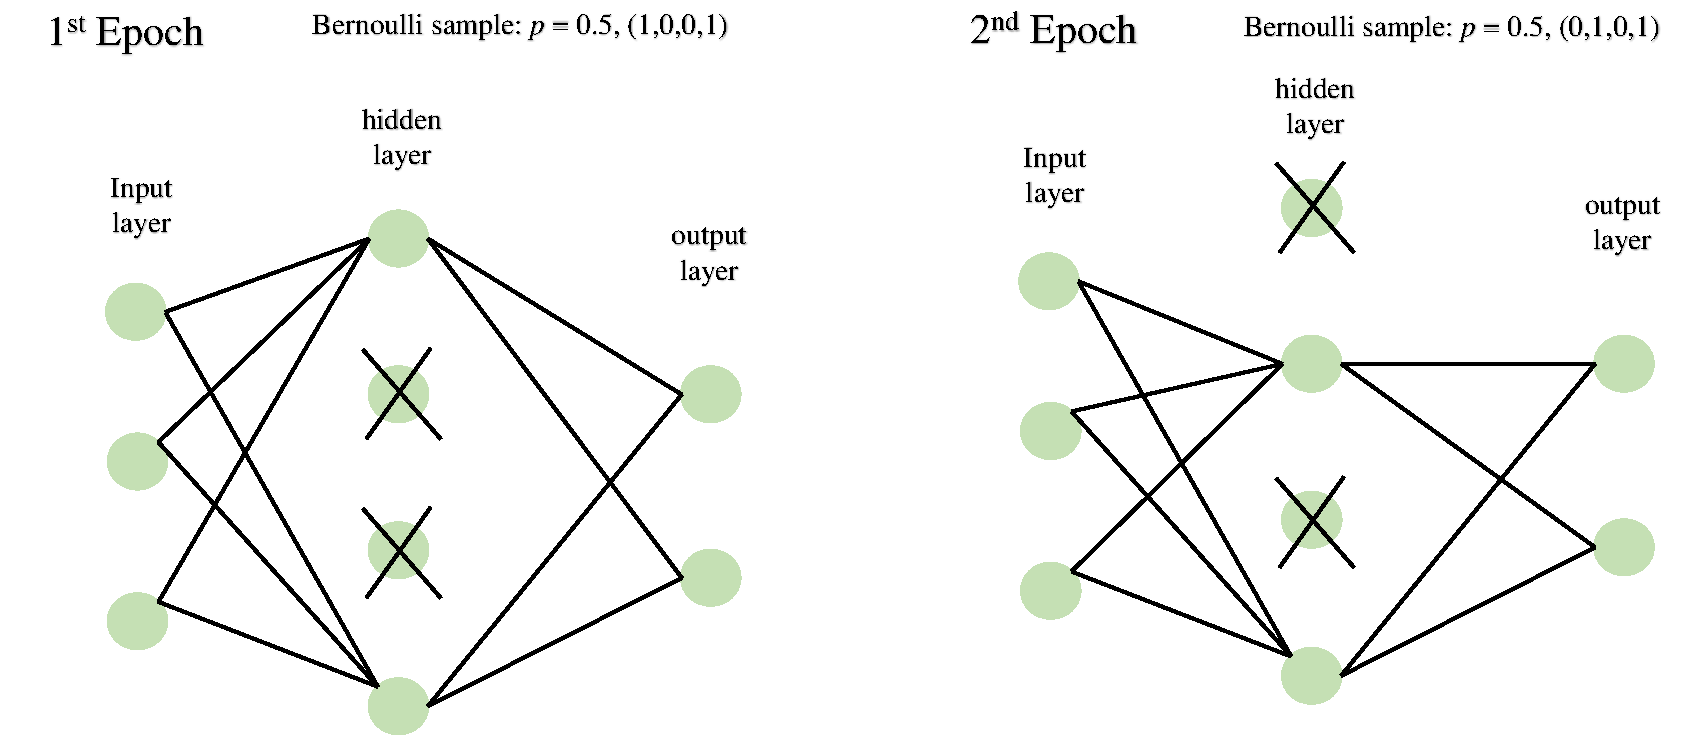
\includegraphics[width=0.8\textwidth]{dropout.pdf} %插入图片,[]中设置图片大小,{}中是图片文件名
\caption{The principle of how dropout works} %最终文档中希望显示的图片标题
\label{fig:dropout} %用于文内引用的标签
\end{figure}
\item[Early stop:]The idea behind early stopping is to monitor the network's performance on a validation set during training and stop the training process once the validation error starts to increase, indicating that the network is starting to overfit the training data.

%\numberwithin{figure}{section}
%\begin{figure}[H] %H为当前位置,!htb为忽略美学标准,htbp为浮动图形
%\centering %图片居中
%\includegraphics[width=0.5\textwidth]{traintest} %插入图片,[]中设置图片大小,{}中是图片文件名
%\caption{Split the data into 2 parts to implement early stop} %最终文档中希望显示的图片标题
%\label{fig:traintest} %用于文内引用的标签
%\end{figure}

In the beginning, the data set is separated into a training set and a validation set randomly. As the network is trained, the training error generally decreases over time, while the validation error initially decreases but then starts to increase again. This is because the network starts to overfit the training data, and the improvements in the training error do not generalize to new data.

\numberwithin{figure}{section}
\begin{figure}[H] %H为当前位置,!htb为忽略美学标准,htbp为浮动图形
\centering %图片居中
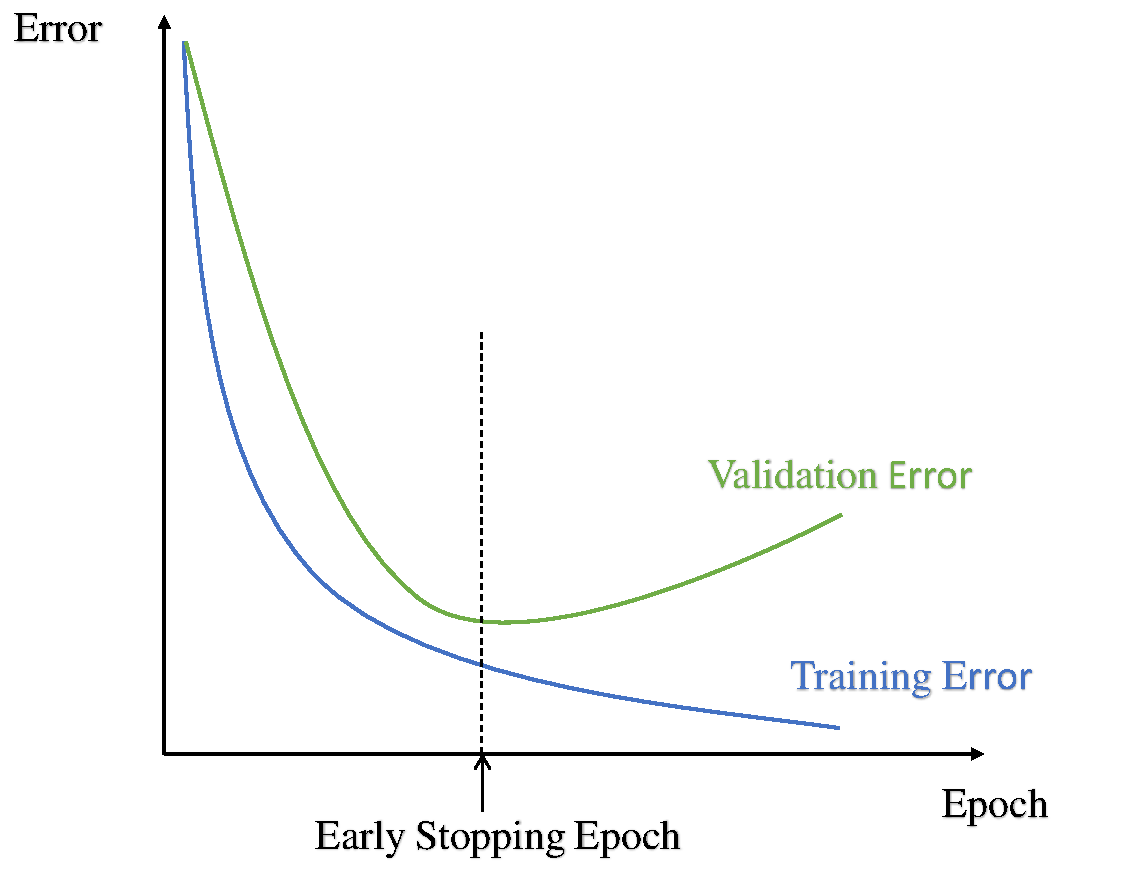
\includegraphics[width=0.6\textwidth]{earlystop.pdf} %插入图片,[]中设置图片大小,{}中是图片文件名
\caption{The principle of how early stop works} %最终文档中希望显示的图片标题
\label{fig:earlystop} %用于文内引用的标签
\end{figure}

The early stopping point is indicated by the dashed line in the graph. This is the point at which the validation error is at its minimum. At this point, the network has achieved the best possible generalization performance on the validation set. Any further training would cause the network to overfit the training data, resulting in worse generalization performance. Therefore, the training process is stopped at the early stopping point, and the network parameters at this point are used as the final trained model. This model has achieved the best possible generalization performance on the validation set and can be used to make predictions on new data.
\end{description}
The following graph shows the training error and validation error in each epoch, and the early stop happened around 54 epochs.

\numberwithin{figure}{section}
\begin{figure}[H] %H为当前位置,!htb为忽略美学标准,htbp为浮动图形
\centering %图片居中
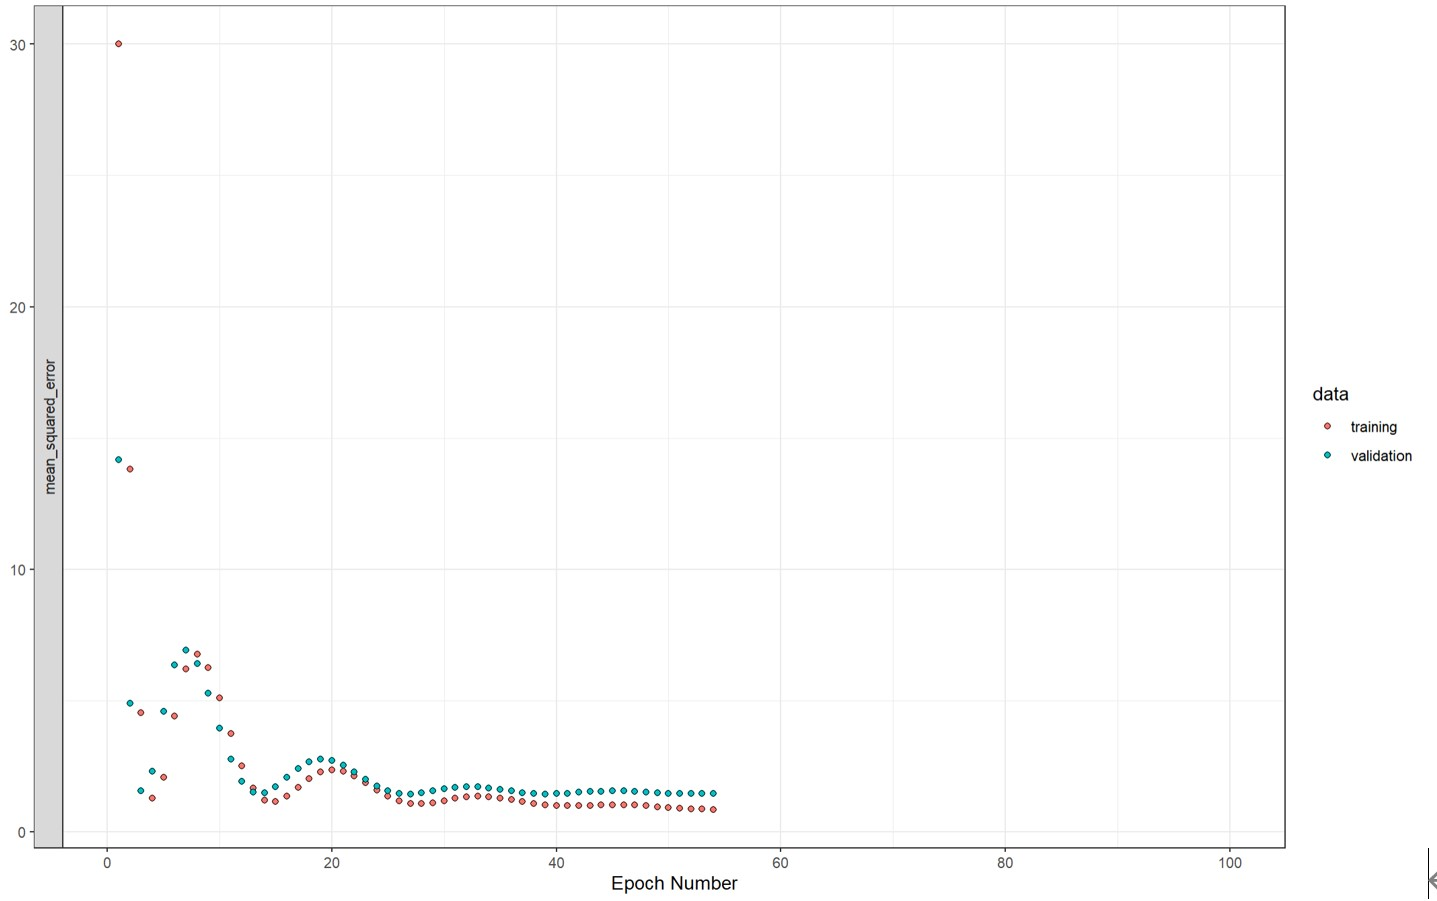
\includegraphics[width=0.7\textwidth]{earlystop example} %插入图片,[]中设置图片大小,{}中是图片文件名
\caption{An example of early stop} %最终文档中希望显示的图片标题
\label{fig:early stop example} %用于文内引用的标签
\end{figure}

\subsection{Autoregression Model}
All the models introduced above try to describe response precipitation with covariates data from the same year as the response. However, this kind of model may not be useful in forecasting, and most of the time it is used to explain the relation between response and covariates. Therefore, we also consider the model predicting next year's response using current year data including observed previous response data. This is what we call the autoregression model (only for naming convenience and has nothing to do with the AR model in time series), using previous years’ response to predict the following years’ response. Here we only consider autoregression on the previous year, namely adding the previous year’s precipitation data as an additional scalar covariate into models. For each model, there are now five functional covariates and one scalar covariate with a total of twenty-three years of data. We will also display and compare the results for this model.

\subsection{Results}
In this subsection, we present the results of all the models stated above, choose $MSE, MSPE$, and $R^2$ as criteria, and give a brief comparison of different models. 
\newpage

\noindent
For the current year regression problem:
\numberwithin{table}{section}
\begin{table}[!htbp]
\centering
\begin{tabular}{cccccc}
   \toprule
   &$Training \quad MSE$ & $MSPE_{cv}$ & $Test\quad MSE$ & $Test\quad R^2$ \\
   \midrule
   FLM without penalty&0.20&---&4.07&-1.83 \\
   FLM with penalty&1.02&1.92&1.43&0.003 \\
   FSR& 0.65&1.28&0.95&0.34\\
   FuncNN&0.33&1.50&0.70&0.51\\
   \bottomrule
\end{tabular}
%\label{table1}
\caption{Result for the current year regression problem}
\end{table}\\
\noindent
For the next year's prediction problem (autoregression):

\numberwithin{table}{section}
\begin{table}[!htbp]
\centering
\begin{tabular}{cccccc}
   \toprule
   &$Training \quad MSE$ & $MSPE_{cv}$ & $Test\quad MSE$ & $Test\quad R^2$ \\
   \midrule
   FLM without penalty&---&---&---&--- \\
   FLM with penalty&1.09&0.89&1.73&-0.20\\
   FSR& 1.02&1.32&1.28&0.11\\
   FuncNN&0.79 &1.48 &1.05 &0.27\\
   \bottomrule
\end{tabular}
%\label{table2}
\caption{Result for the next year prediction problem}
\end{table}
\noindent 
From the above results, we can make the following conclusions:
\begin{itemize}
\item[a.] Comparing the FLM with penalty term and without penalty term:

The FLM without penalty term can be overfitting (train MSE is much smaller than test MSE) and adding a penalty term for the functional linear model can ease overfitting, as well as decrease the test MSE and increase test $R^2$, i.e., improve performance of the model. However, its test $R^2$ is approximately 0, which means the performance is still not good.
\item[b.] Comparing the FLM using the original 5 covariates and the FLM with 3 PCs:

Both two models add a penalty term, the test MSE of the FLM with PCs is lower and the test $R^2$ increased by 0.3, indicating the performance of FLM using PCs is much better.
\item[c.] Comparing the FuncNN with all the other models:

The test MSE of the FuncNN is the lowest and its test $R^2$ is the highest, which means FuncNN performs best among all the models stated in this paper.
\item[d.] Comparing all the regression models for the current year and all the prediction models for the next year (autoregression models):

The test MSE of the regression models is much smaller than the autoregression models, and this result is different from the guess we had in section 3.6. We suggest that maybe this data set is not suitable for the autoregression model.
\end{itemize}
\section{Discussion}
Functional data analysis has been a hot topic in recent years, and its wide adaptability makes it worthwhile for further investigation. However, deep learning with functional data analysis is still at its initial stage and more effort needs to be done to complete the system of functional data analysis both in theories and applications. In our project, we first reviewed some important concepts of functional data analysis, comparing those in the traditional multivariate fields. These concepts include techniques for smoothing, FPCA, and also functional linear models. A byproduct, functional score regression which applies PCA on multivariate perspectives but regression on a functional linear model, was introduced.  Apart from the functional linear model, we have also considered neural networks on functional data, putting forward ideas to implement neural networks on functional data. After finishing the reviews on concepts, we did apply those techniques in real data, trying to explain average annual precipitation in Macau SAR with five functional covariates including daily average temperature, daily average relative humidity, daily average wind speed, daily average sea level pressure, and daily total sunshine duration. Comparing the results of the models, we figured out that FuncNN performed best in this data set. We guessed the reason is that the relation between precipitation and those five covariates may not be linear and neural network has some advantages in dealing with nonlinear relations than linear models. From the result, we see the excellent performance of neural networks on functional data, even though functional neural network analysis is still in its infancy stage. It is worthy of developing the field of functional neural networks.

During our experiment, we did also discover something worth thinking about. First of all, the performance of functional data analysis may heavily depend on the smoothing of functional data, while there are few formal criteria to choose the number of basic functions. Secondly, the collinearity of covariates may result in poor performance of models but there are not enough methods to deal with this problem. Thirdly, as far as we are concerned, there did not exist a normative significance test of functional coefficients like those in multivariate analysis. Finally, the functional neural network used here is essentially a method in scalar space, only performing transformation from functional data into the first layer, remaining the hidden layers the same as traditional ones. To apply to a wider range of scenarios, we shall investigate neurons in functional space. 

In summary, the experiment presented here first reviewed theories in functional data analysis, introducing FLM and FuncNN, then implemented models in real data sets, revealing some directions for further works. Functional data analysis is powerful, and it is necessary to perfect the system of analysis.




